\documentclass{article}

\usepackage[T1]{fontenc}
\usepackage[utf8]{inputenc}
\usepackage[brazilian]{babel}
\usepackage{graphicx}
\usepackage[export]{adjustbox}[2011/08/13]
\usepackage{float}
\usepackage[pdftex]{hyperref}
\usepackage{epstopdf}
\usepackage{etoolbox}
\usepackage{amsmath}
\usepackage{amsfonts}
\usepackage{amssymb}
\usepackage{caption}
\usepackage{subcaption}
\usepackage{setspace}
\usepackage{tikz}
\usepackage{listings}
\usepackage{xcolor} 

\bibliographystyle{eric}
\patchcmd{\thebibliography}{\section*}{\section}{}{}


\newcommand{\R}{\ensuremath{\mathbb{R}}}
\newcommand{\Prob}{\ensuremath{\mathbb{P}}}
\newcommand{\K}{\ensuremath{\mathbb{K}}}
\newcommand{\U}{\ensuremath{\mathbb{U}}}
\newcommand{\N}{\ensuremath{\mathbb{N}}}
\newcommand{\Lg}{\ensuremath{\mathbb{L}}}
\newcommand{\T}{\ensuremath{\rm Tr}}
\newcommand{\sg}{{\sigma(x_k)}}

\newcommand{\G}{\ensuremath{\mathcal{G}}}
\newcommand{\F}{\ensuremath{\mathcal{F}}}
\newcommand{\C}{\ensuremath{\mathcal{C}}}
\newcommand{\E}{\ensuremath{\mathcal{E}}}
\newcommand{\Hn}{\ensuremath{\mathcal{H}}}
\newcommand{\Hoo}{\ensuremath{\mathcal{H}_\infty}}
\newcommand{\Hop}{\ensuremath{\mathcal{H}_{op}}}
% --------------------------------------------------
\newtheorem{theo}{Teorema}
\newtheorem{exa}{Exemplo}
\newtheorem{lemm}{Lema}
\newtheorem{coro}{Corolário}
\newtheorem{defn}{Definição}[section]

\begin{document}

\begin{titlepage}
\begin{center}

\newcommand{\HRule}{\rule{\linewidth}{0.5mm}}
% Upper part of the page. The '~' is needed because \\
% only works if a paragraph has started.

\includegraphics[width=0.15\textwidth]{logoUnicamp}~\\[1cm]

\textsc{\LARGE Universidade Estadual de Campinas}\\[1.5cm]

\textsc{\Large Faculdade de Engenharia Mecânica}\\[0.5cm]

% Title
\HRule \\[0.4cm]
{ \huge \bfseries ES664 - Laboratório de Eletrônica para Automação Industrial\\ \vspace{1cm} Relatório - Experimento 4\\
\Large{Acionamento de motor DC} \\[0.4cm] }

\HRule \\[1.5cm]

% Author and supervisor
\begin{minipage}{0.6\textwidth}
\begin{flushleft} \large
\emph{Nome:}\\
Daniel Dello Russo Oliveira\\Marcelli Tiemi Kian
\end{flushleft}
\end{minipage}
\begin{minipage}{0.2\textwidth}
\begin{flushright} \large
\emph{RA}\\ 101918\\117892
\end{flushright}
\end{minipage}

\vfill

% Bottom of the page
{\large \today}

\end{center}
\end{titlepage}


\onehalfspacing
\section{Objetivos}
	Essa simulação tem como objetivo o estudo dos motores DC de ímãs permanentes e sua acionamento através de topologias baseadas em retificadores controlados.
	 
\section{Simualações}
\subsection{Modelagem de um motor DC: diagrama de blocos}
Através do Simulink implementamos a função de transferência de um motor DC através do diagrama de blocos apresentado na figura \ref{fig:sim1}.
\begin{figure}[H]
	\centering
	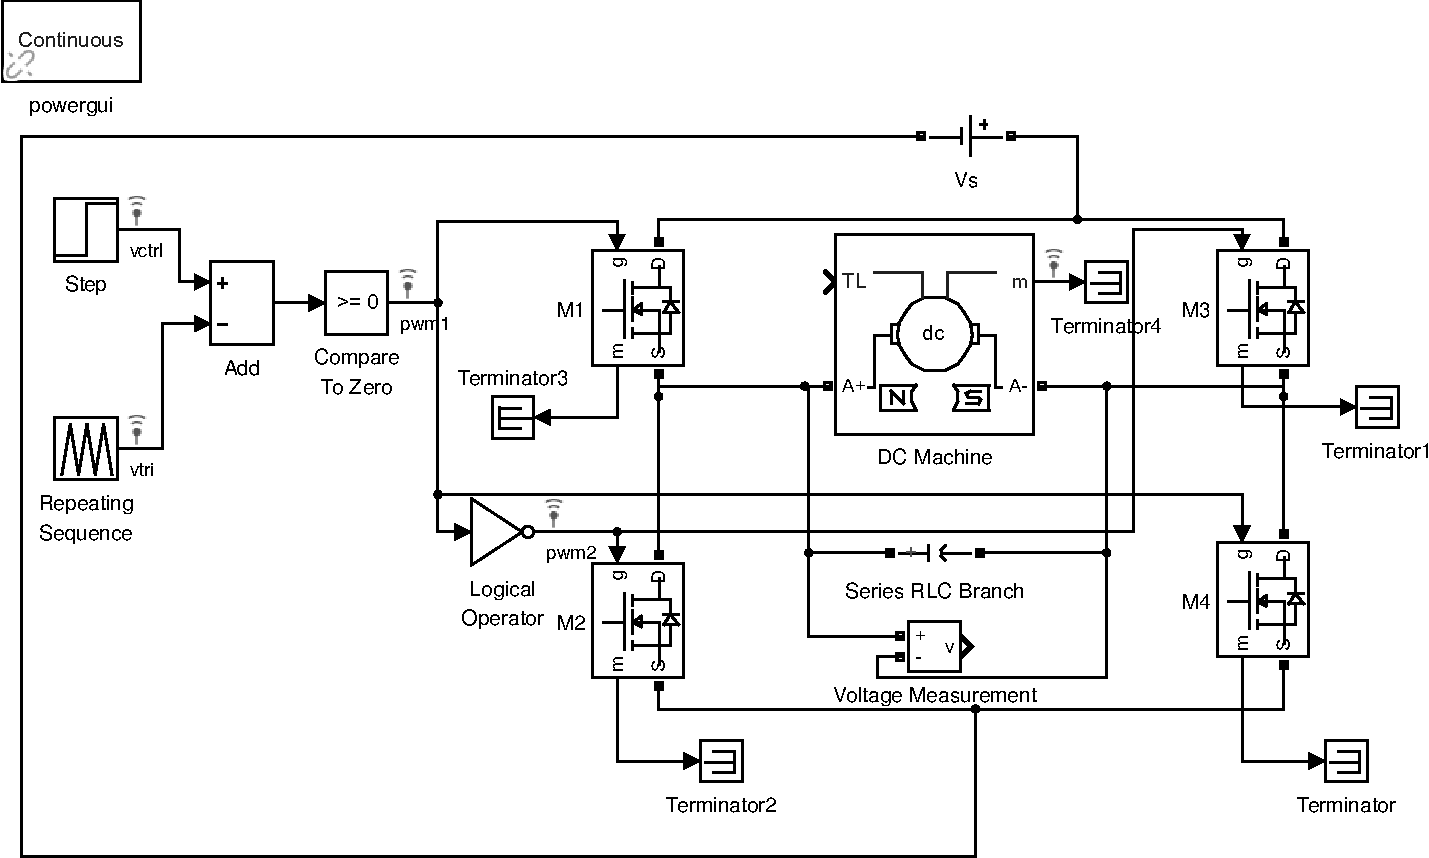
\includegraphics[width=\linewidth]{matlab/sim1}
	\caption{Motor DC implementado através do diagrama de blocos}
	\label{fig:sim1}
\end{figure}
Separamos a parte elétrica e mecânica da função de transferência do motor conforme pode ser visto na figura. Adotamos os valores apresentados no roteiro para os parâmetros do motor ($R_a = 1.6 \Omega$, $L_a = 667 \mu H$, $J = 1.1 \times 10^{-4} kg\ m^2$, $B = 1.24 \times 10^{-4} J\ s/rad$, $k_e = 0.038 V\ s/rad$ e $k_t = 0.038 N\ m/A$).

Simulamos a resposta do motor sem carga a um degrau de 24V obtendo as curvas apresentadas na figura \ref{fig:res1}

\begin{figure}[H]
	\centering
	\begin{subfigure}[b]{0.49\linewidth}
		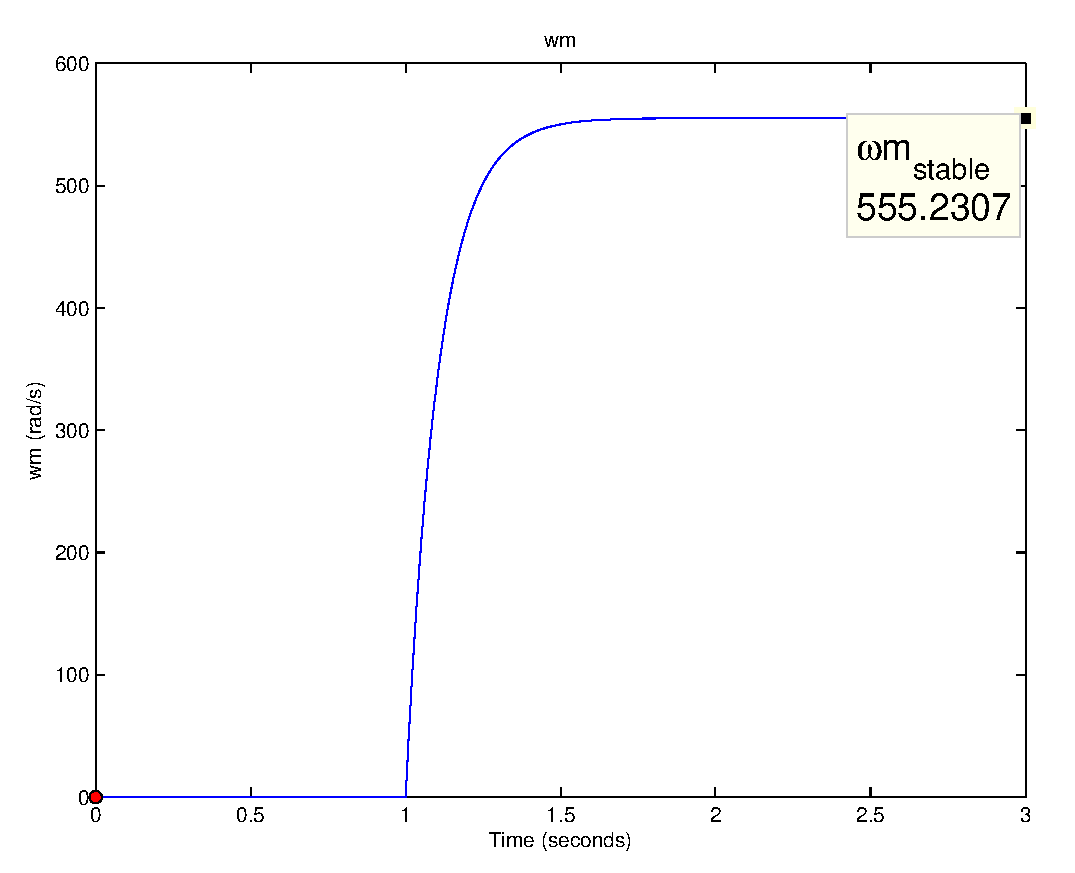
\includegraphics[width=\linewidth]{matlab/wm1}
		\caption{Velocidade Angular}
	\end{subfigure}
	\begin{subfigure}[b]{0.49\linewidth}
		\centering
		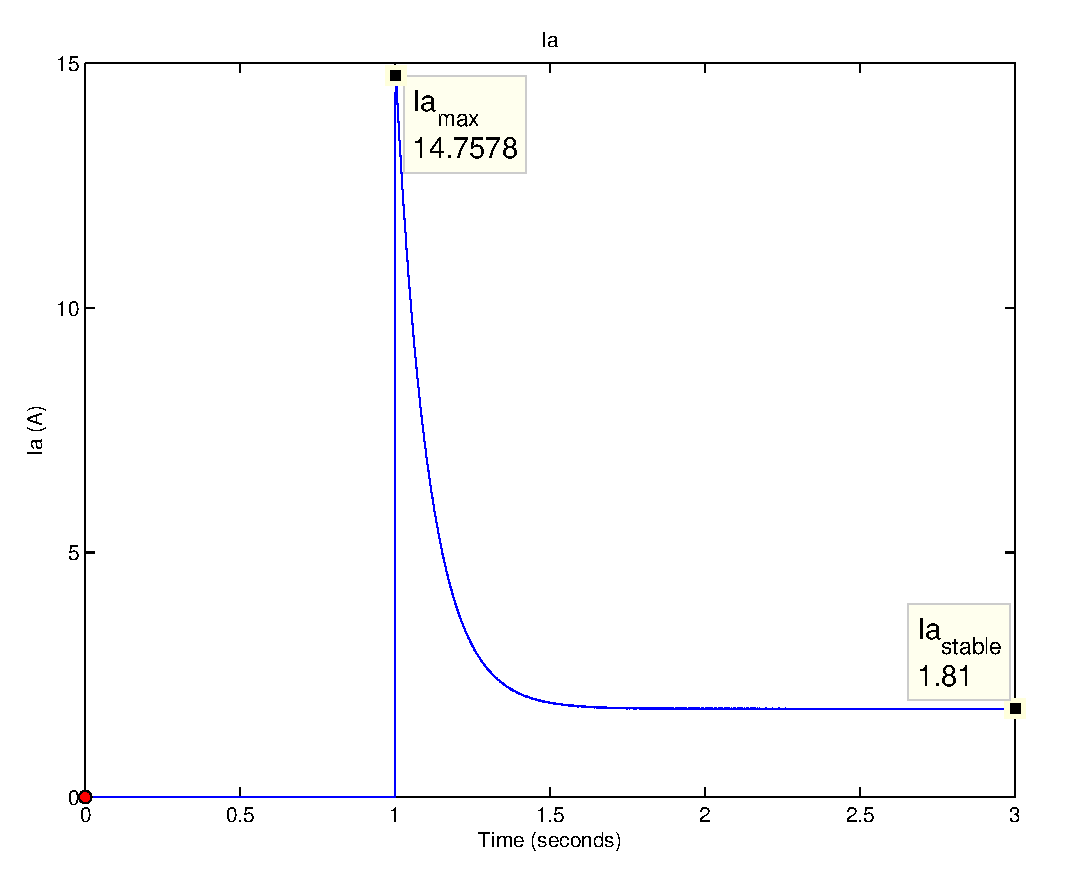
\includegraphics[width=\linewidth]{matlab/ia1}
		\caption{Corrente de armadura}
	\end{subfigure}
	\begin{subfigure}[b]{0.49\linewidth}
		\centering
		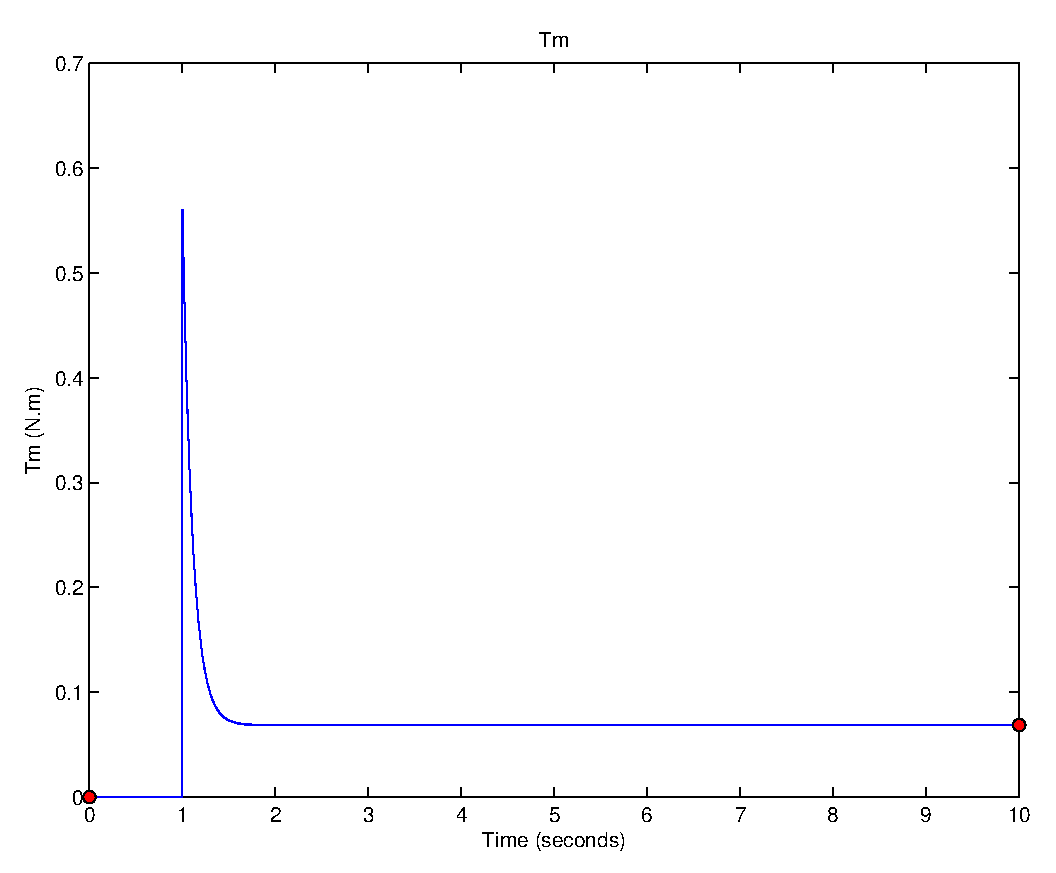
\includegraphics[width=\linewidth]{matlab/tm1}
		\caption{Torque do motor}
	\end{subfigure}
	\caption{Curvas de resposta do motor sem carga}
	\label{fig:res1}
\end{figure}

Colocamos então uma carga proporcional à velocidade no nosso motor (de função $Twl = - 5\times10^{-4}\omega_m$) e simulamos a resposta do motor ao mesmo degrau de entrada, obtendo as curvas da figura \ref{fig:res2}

\begin{figure}[H]
	\centering
	\begin{subfigure}[b]{0.49\linewidth}
		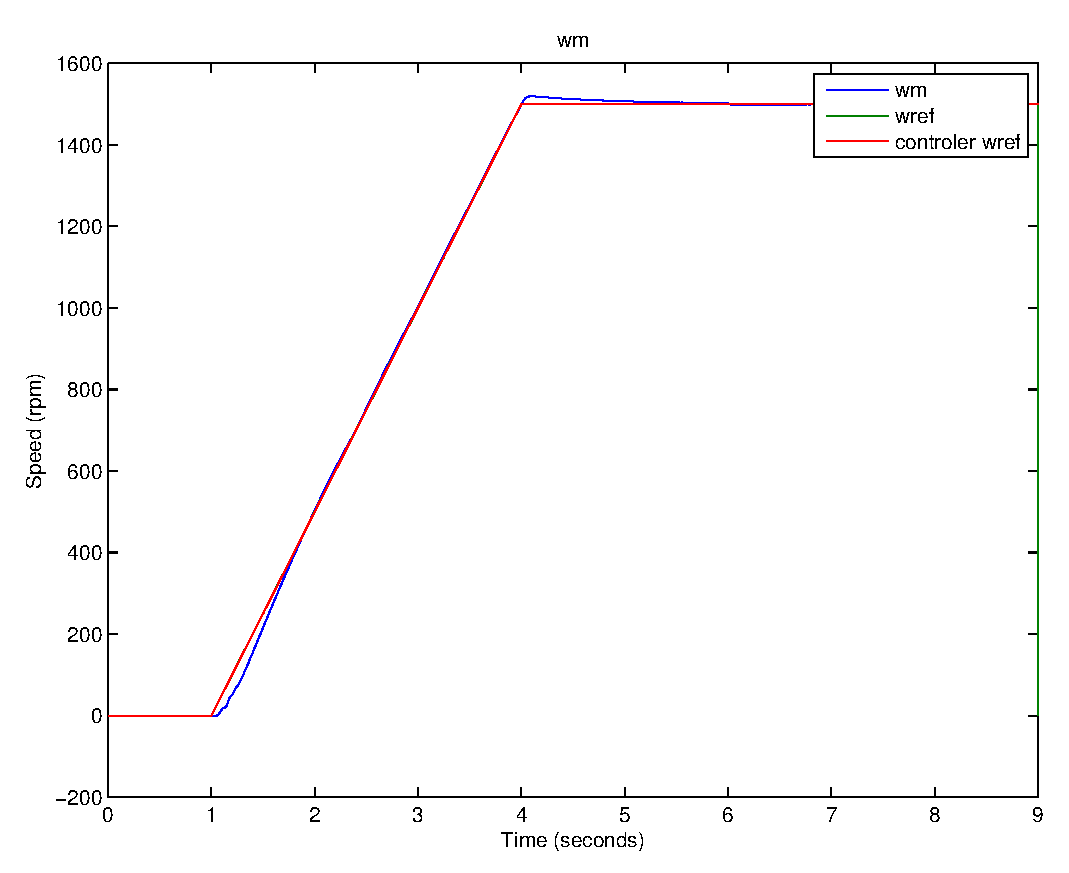
\includegraphics[width=\linewidth]{matlab/wm2}
		\caption{Velocidade Angular}
	\end{subfigure}
	\begin{subfigure}[b]{0.49\linewidth}
		\centering
		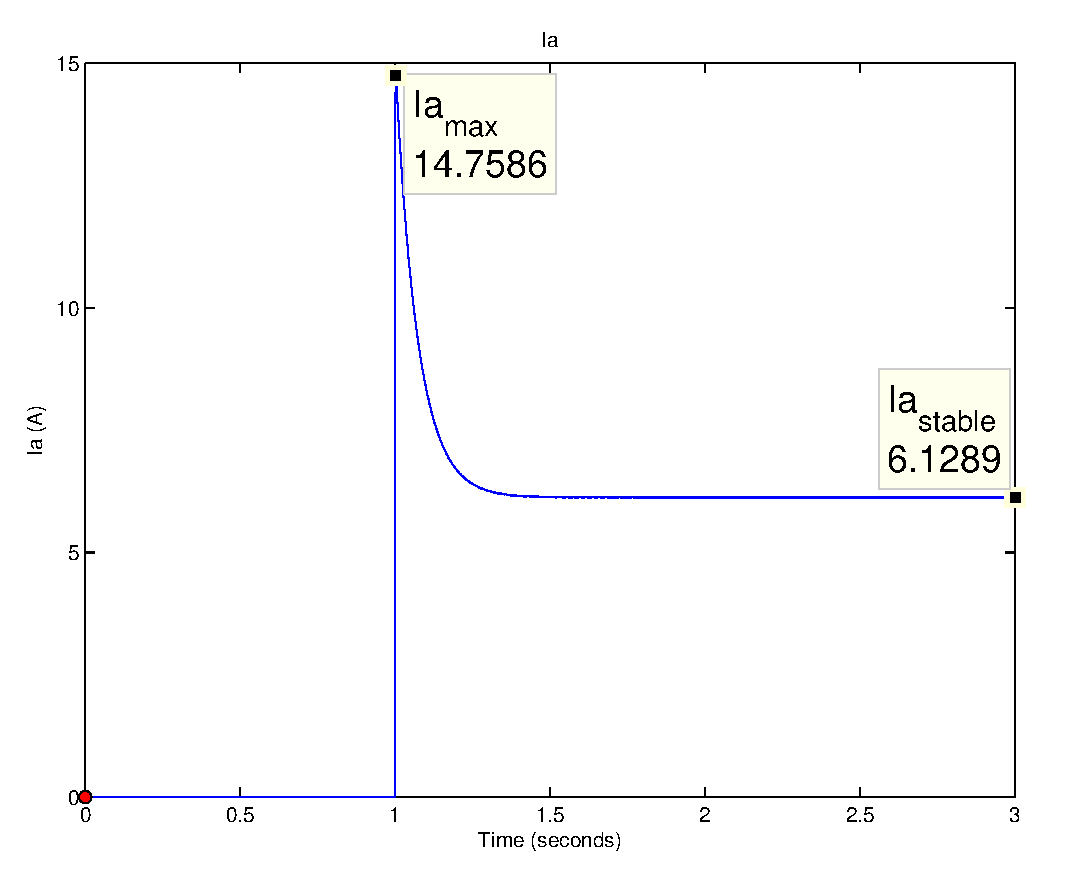
\includegraphics[width=\linewidth]{matlab/ia2}
		\caption{Corrente de armadura}
	\end{subfigure}
	\begin{subfigure}[b]{0.49\linewidth}
		\centering
		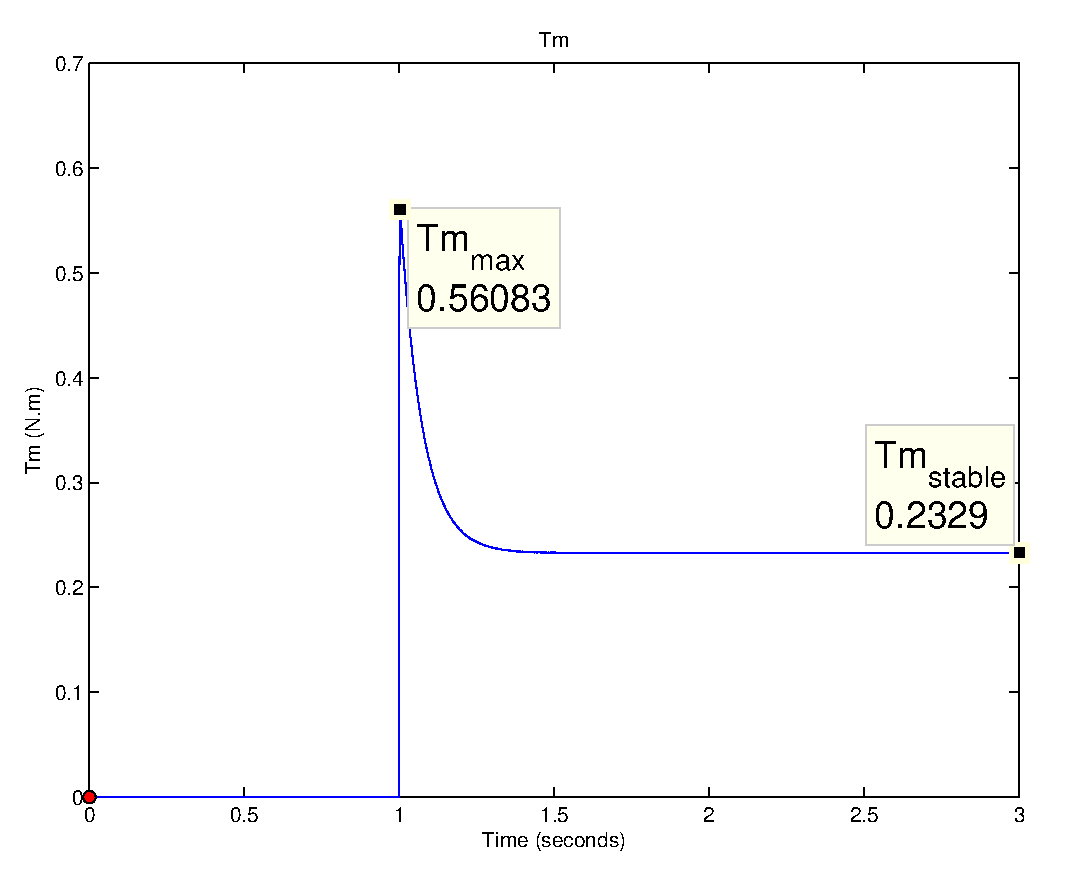
\includegraphics[width=\linewidth]{matlab/tm2}
		\caption{Torque do motor}
	\end{subfigure}
	\caption{Curvas de resposta do motor com carga proporcional à velocidade}
	\label{fig:res2}
\end{figure}

Notamos que a corrente não aumentou, porém o torque de saída aumentou enquanto a velocidade diminuiu.

\subsection{Modelagem de um motor DC: SimPowerSystems}
Utilizando a biblioteca SimPowerSystems do Simulink implementamos o mesmo motor DC, agora utilizando o modelo disponível na biblioteca, conforme apresentado na figura \ref{fig:sim2}.
\begin{figure}[H]
	\centering
	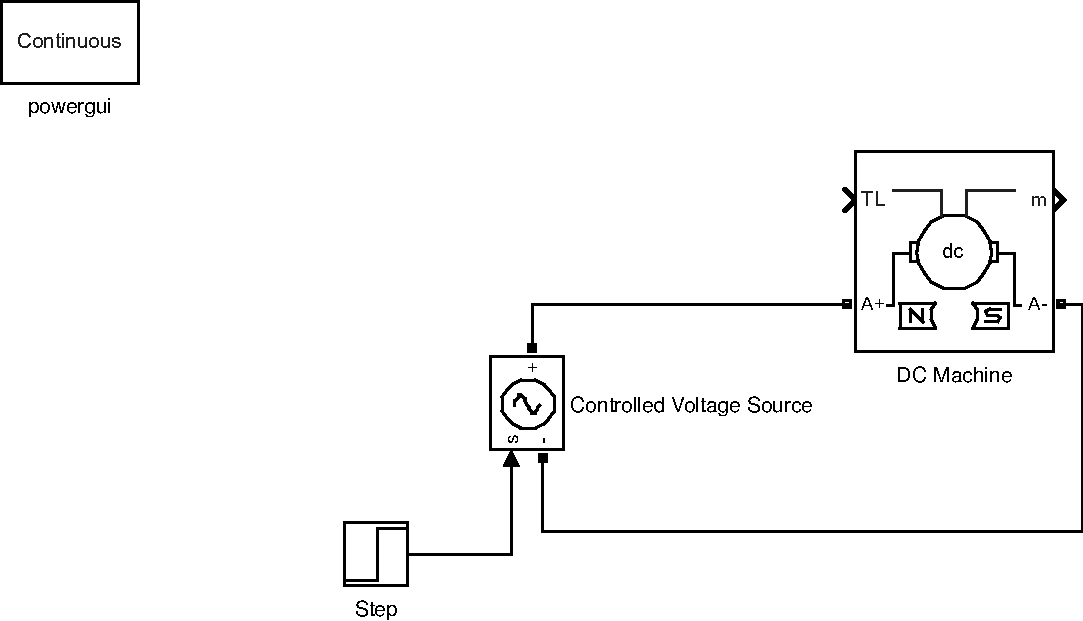
\includegraphics[width=0.6\linewidth]{matlab/sim2}
	\caption{Motor DC implementado através da biblioteca SimPowerSystems}
	\label{fig:sim2}
\end{figure}

Simulamos a resposta do motor sem carga a o mesmo degrau de 24V obtendo as curvas apresentadas na figura \ref{fig:res3}

\begin{figure}[H]
	\centering
	\begin{subfigure}[b]{0.49\linewidth}
		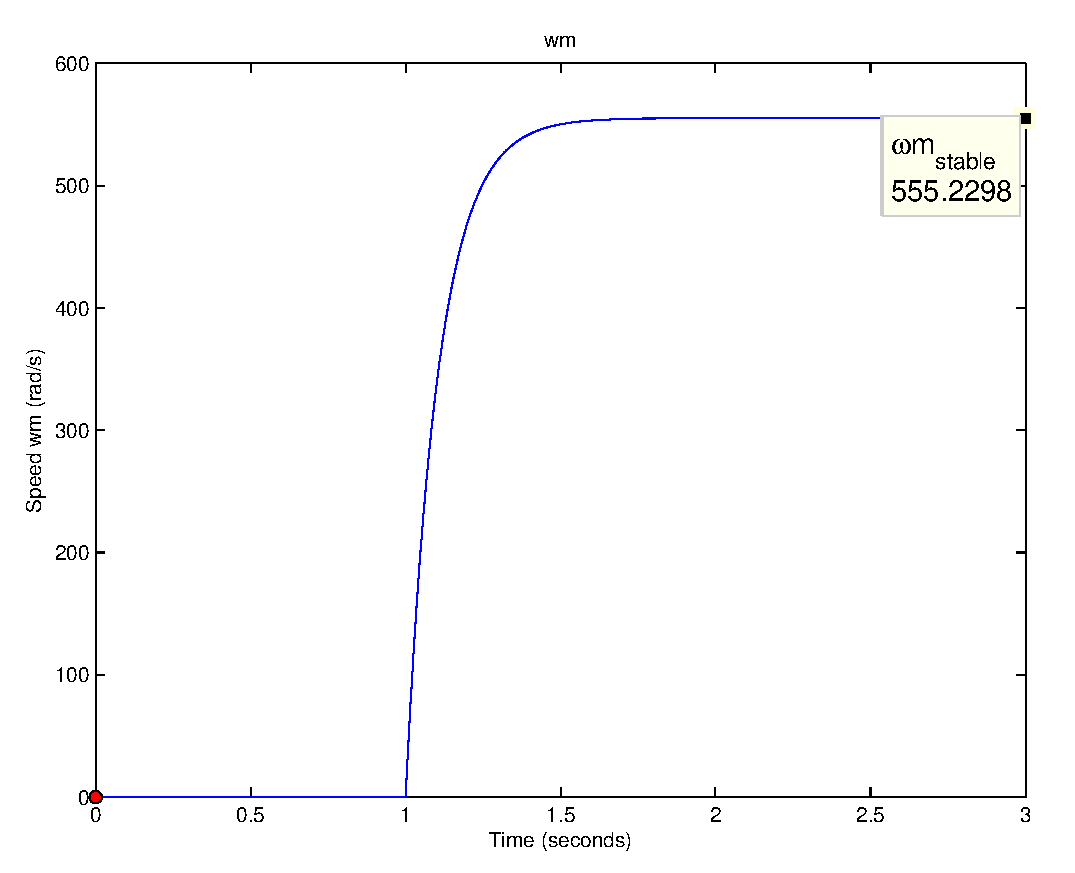
\includegraphics[width=\linewidth]{matlab/wm3}
		\caption{Velocidade Angular}
	\end{subfigure}
	\begin{subfigure}[b]{0.49\linewidth}
		\centering
		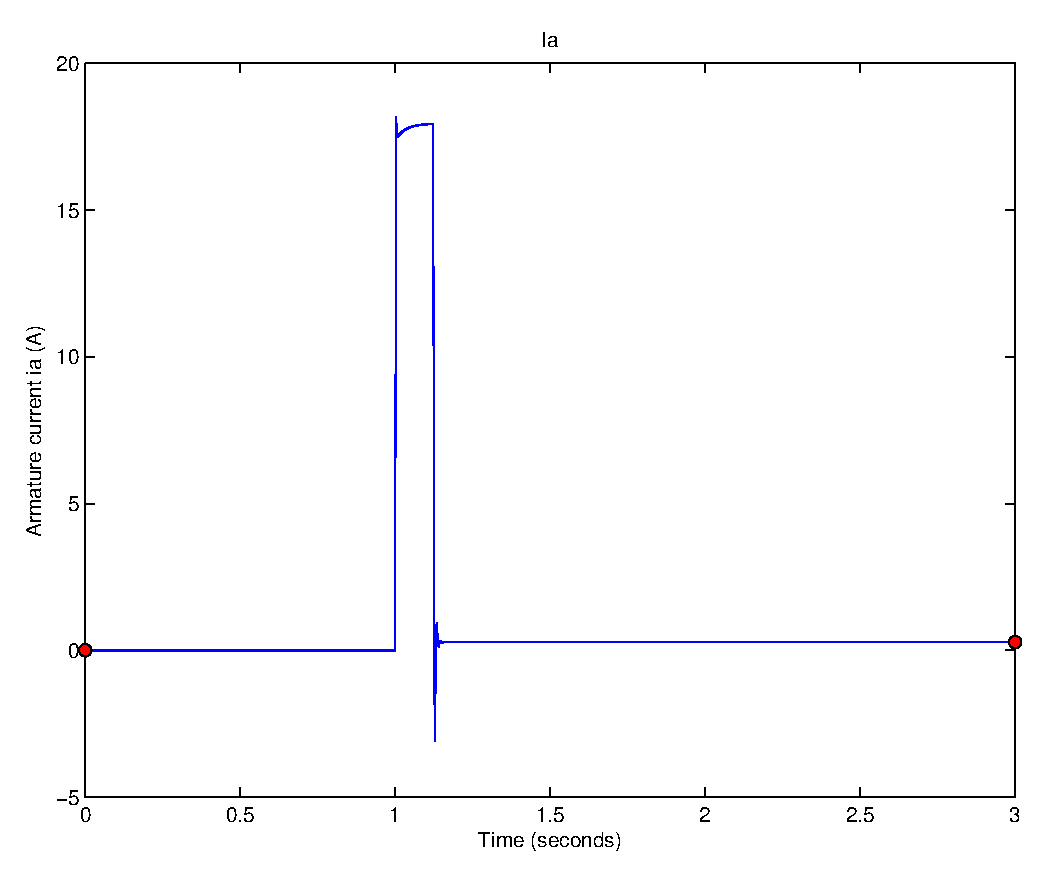
\includegraphics[width=\linewidth]{matlab/ia3}
		\caption{Corrente de armadura}
	\end{subfigure}
	\begin{subfigure}[b]{0.49\linewidth}
		\centering
		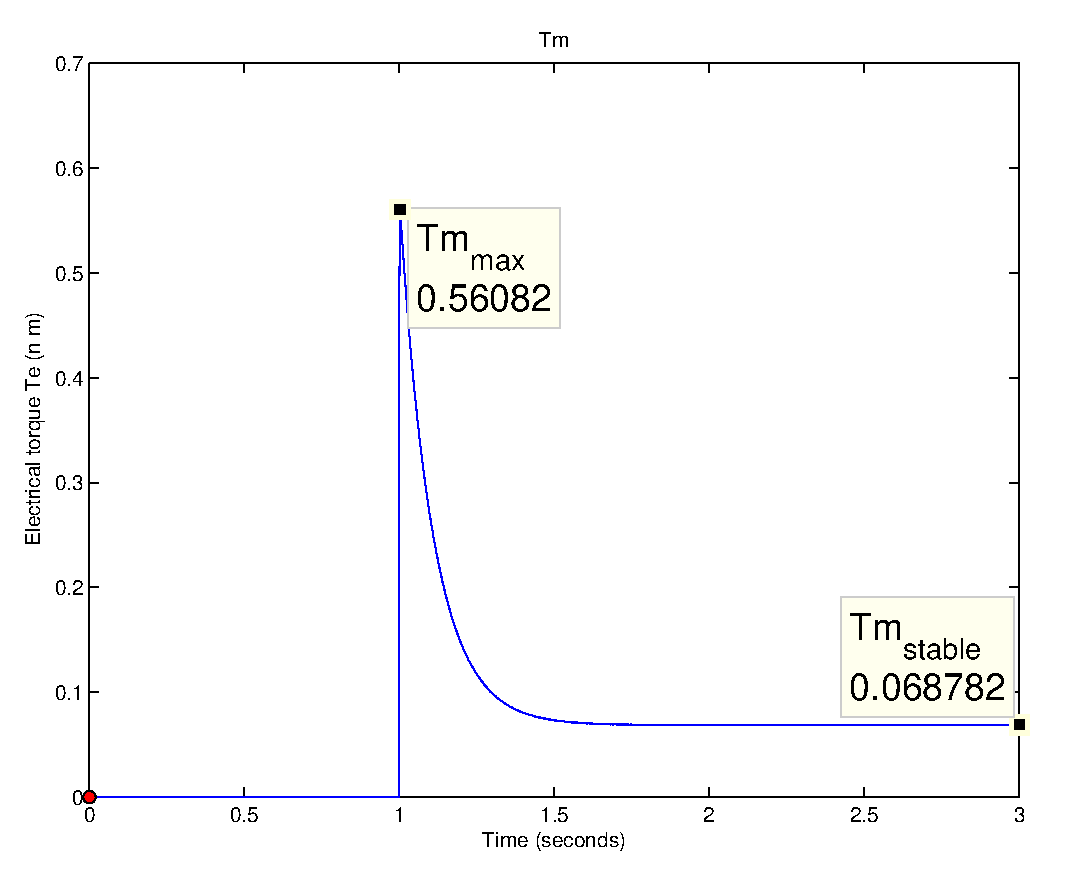
\includegraphics[width=\linewidth]{matlab/tm3}
		\caption{Torque do motor}
	\end{subfigure}
	\caption{Curvas de resposta do motor sem carga}
	\label{fig:res3}
\end{figure}

Como podemos ver os resultados são bastante semelhantes aos apresentados na figura \ref{fig:res1}, se não praticamente idênticos. Como podemos ver nosso modelo por blocos e o modelo utilizado internamente pela biblioteca são bastante semelhantes.

\subsection{Acionamento de motor DC com retificador controlado}
Conectamos um retificador monofásico controlado de onda completa no nosso motor alimentado por uma fonte alternada (24 V rms@60 Hz), conforme pode ser visto na figura \ref{fig:sim3}.
\begin{figure}[H]
	\centering
	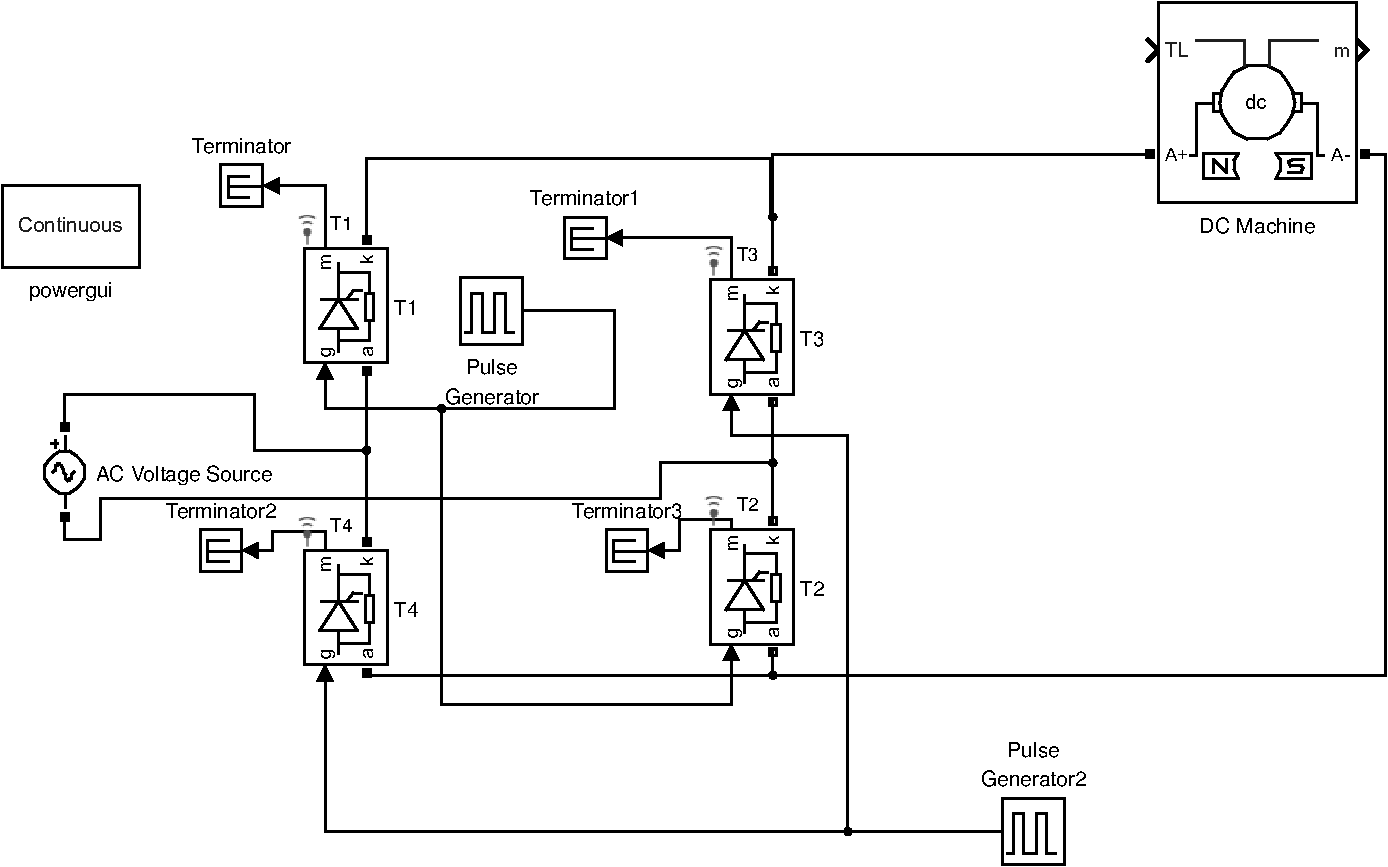
\includegraphics[width=\linewidth]{matlab/sim3}
	\caption{Acionamento de motor DC através de retificador monofásico controlado}
	\label{fig:sim3}
\end{figure}

Simulamos a resposta do motor para ângulos de disparo de $0^\circ$ (figura \ref{fig:res4}) e $90^\circ$ (figura \ref{fig:res5}).

\begin{figure}[H]
	\centering
	\begin{subfigure}[b]{0.49\linewidth}
		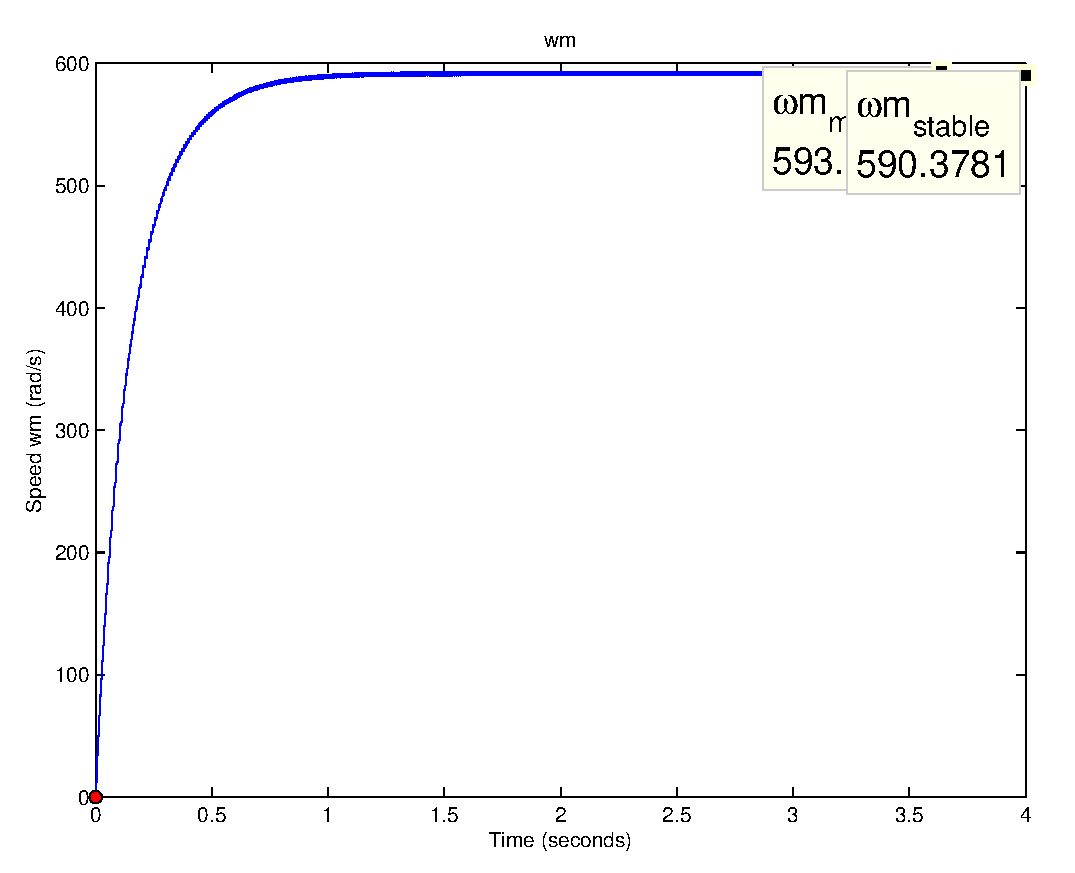
\includegraphics[width=\linewidth]{matlab/wm4}
		\caption{Velocidade Angular}
	\end{subfigure}
	\begin{subfigure}[b]{0.49\linewidth}
		\centering
		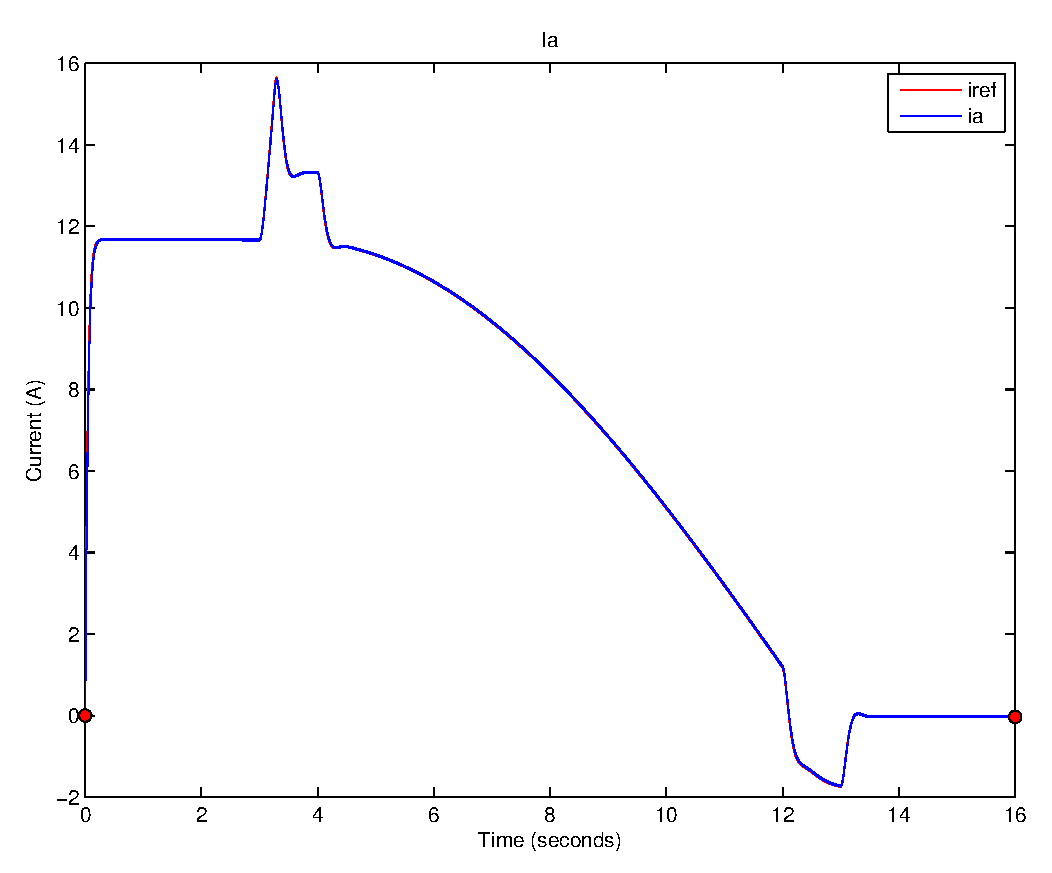
\includegraphics[width=\linewidth]{matlab/ia4}
		\caption{Corrente de armadura}
	\end{subfigure}
	\begin{subfigure}[b]{0.49\linewidth}
		\centering
		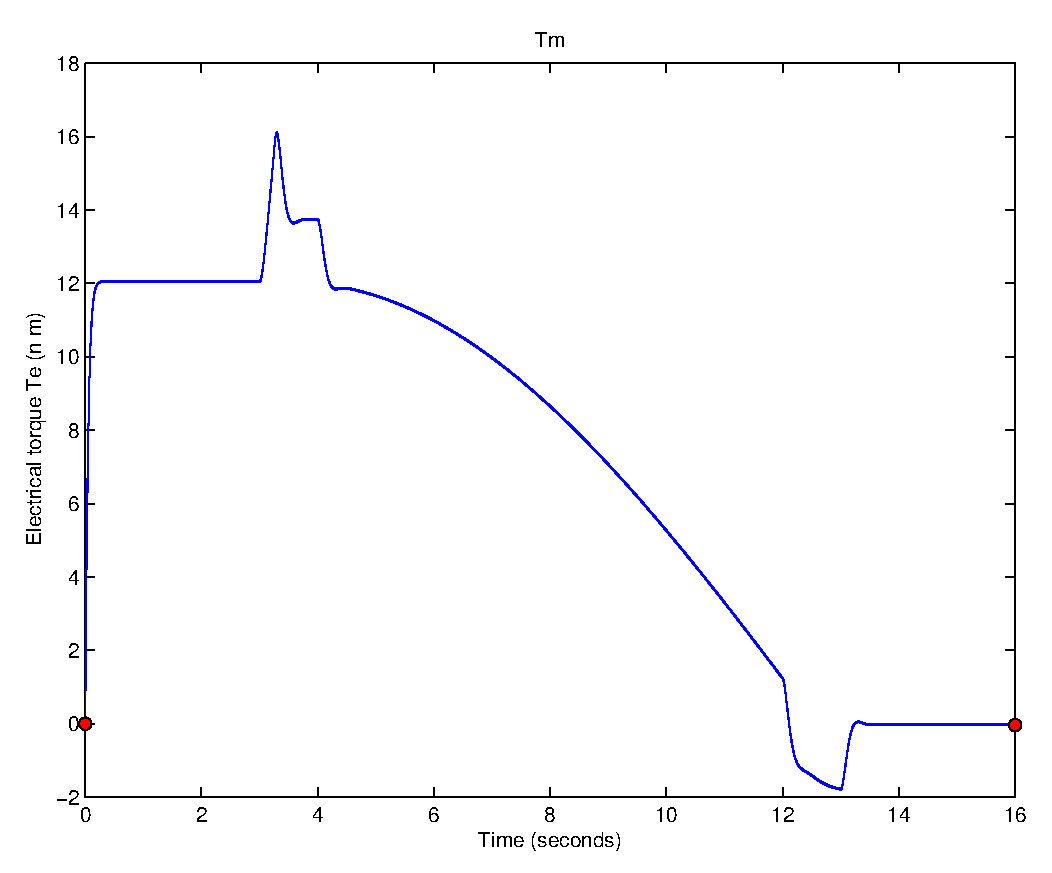
\includegraphics[width=\linewidth]{matlab/tm4}
		\caption{Torque do motor}
	\end{subfigure}
	\caption{Curvas de resposta do motor ângulo de disparo $0^\circ$}
	\label{fig:res4}
\end{figure}

\begin{figure}[H]
	\centering
	\begin{subfigure}[b]{0.49\linewidth}
		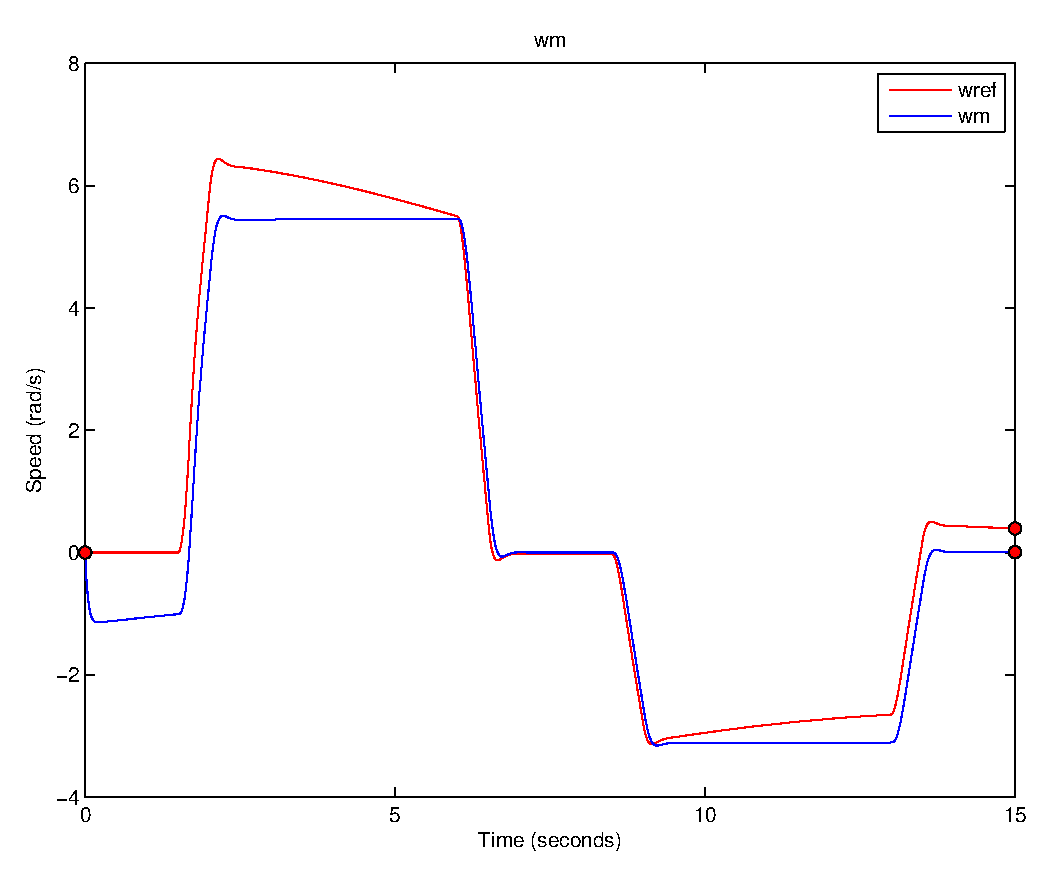
\includegraphics[width=\linewidth]{matlab/wm5}
		\caption{Velocidade Angular}
	\end{subfigure}
	\begin{subfigure}[b]{0.49\linewidth}
		\centering
		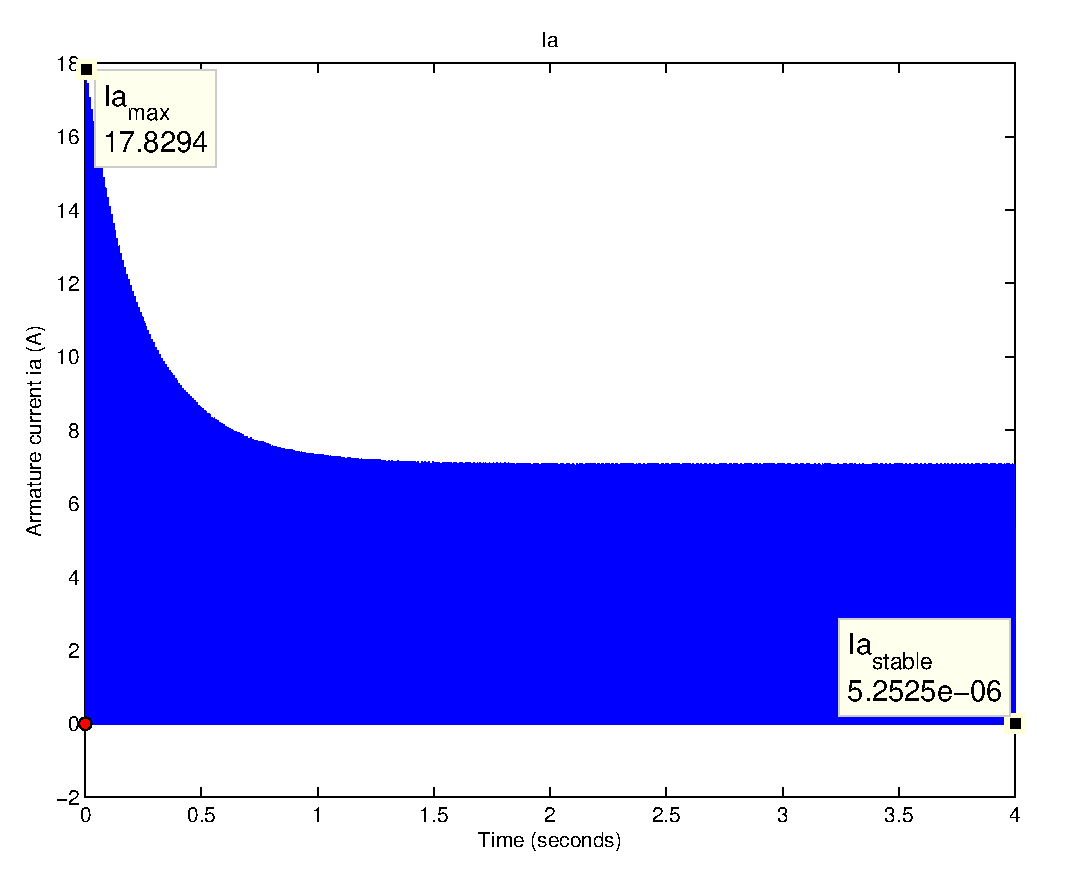
\includegraphics[width=\linewidth]{matlab/ia5}
		\caption{Corrente de armadura}
	\end{subfigure}
	\begin{subfigure}[b]{0.49\linewidth}
		\centering
		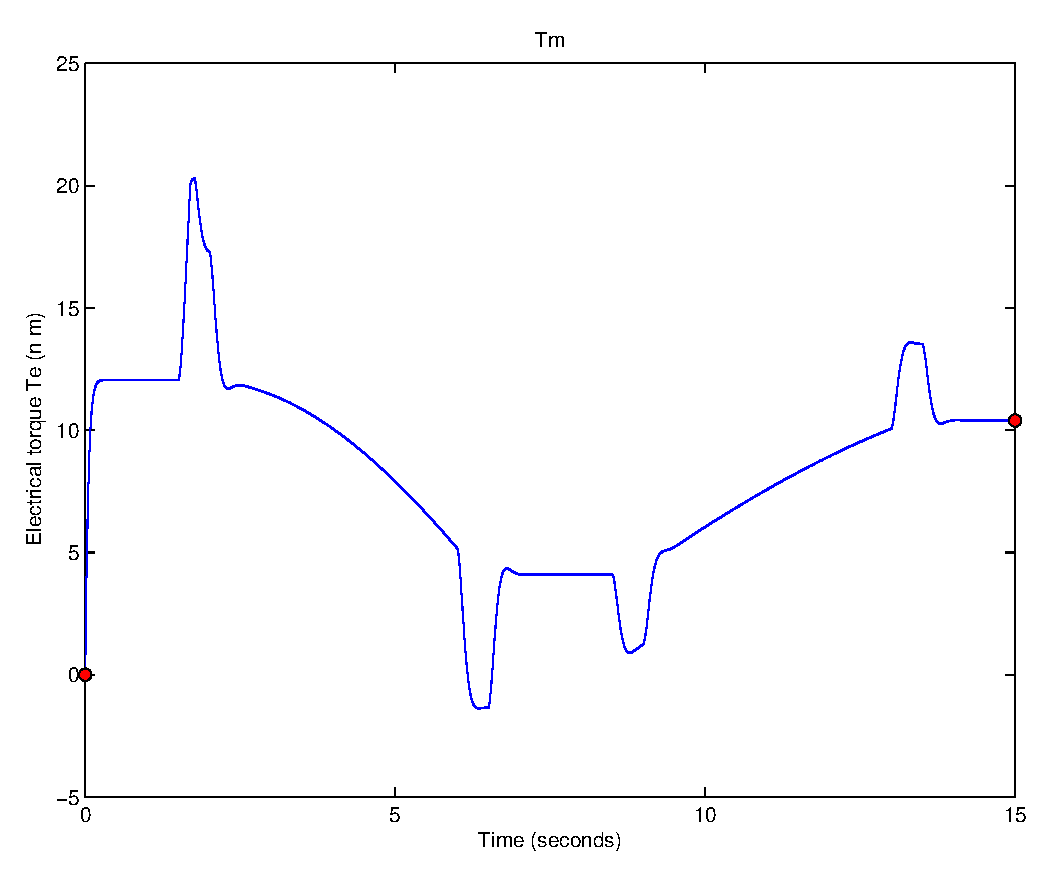
\includegraphics[width=\linewidth]{matlab/tm5}
		\caption{Torque do motor}
	\end{subfigure}
	\caption{Curvas de resposta do motor ângulo de disparo $90^\circ$}
	\label{fig:res5}
\end{figure}
Como podemos ver a oscilação de tensão gerada pelo retificador não pode ser sentida na velocidade do motor, porém ela afeta fortemente a corrente de armadura e o torque de saída. Também notamos que o efeito da mudança do ângulo de disparo é muito pequeno, mudando somente o tempo de resposta do circuito. Acreditamos que isso ocorre pois o motor encontra-se já saturado em ambas as configurações. Mudamos a fonte de 24 V rms para tensão de pico 24 V e rodamos as simulações novamente, obtendo as curvas de velocidade apresentadas na figura \ref{fig:res9}

\begin{figure}[H]
	\centering
	\begin{subfigure}[b]{0.49\linewidth}
		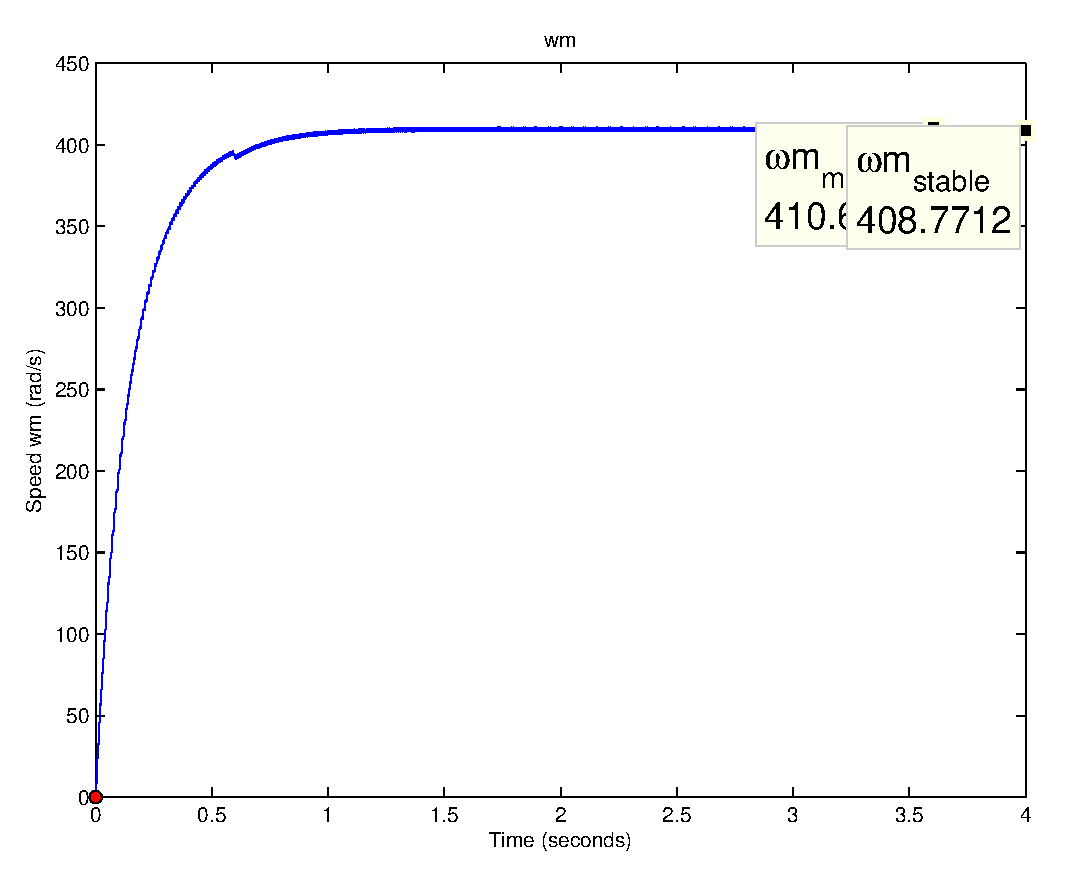
\includegraphics[width=\linewidth]{matlab/wm9}
		\caption{$0^\circ$}
	\end{subfigure}
	\begin{subfigure}[b]{0.49\linewidth}
		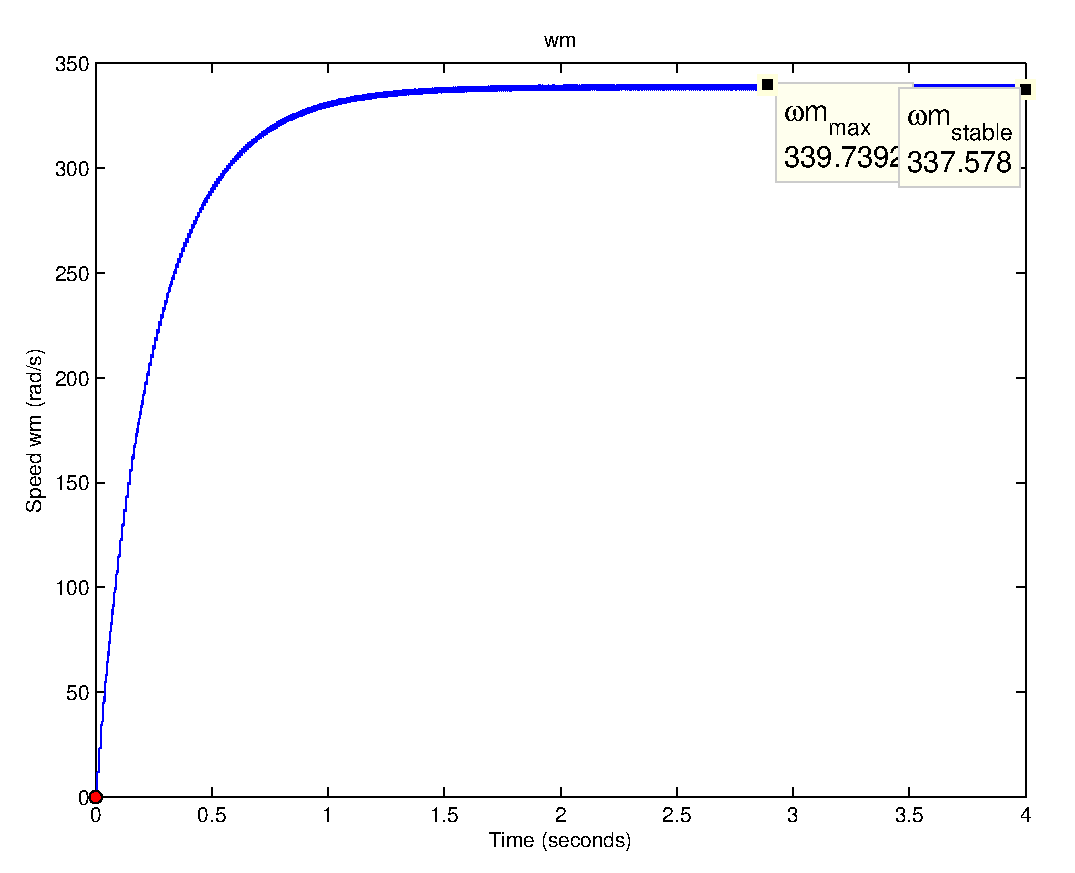
\includegraphics[width=\linewidth]{matlab/wm10}
		\caption{$90^\circ$}
	\end{subfigure}
	\caption{Velocidade do motor para diferentes ângulos de disparo}
	\label{fig:res9}
\end{figure}

Como podemos ver, agora o ângulo de disparo tem uma influência considerável na velocidade atingida pelo motor, conforme o esperado uma vez que ao alterar esse ângulo estamos alterando a tensão de armadura média aplicada.

Para resolver o problema das oscilações na corrente de armadura e no torque, conectamos um filtro capacitivo em nosso sistema (através de um capacitor de $0.5 F$ conectado em paralelo ao motor), conforme apresentado na figura \ref{fig:sim4} 

\begin{figure}[H]
	\centering
	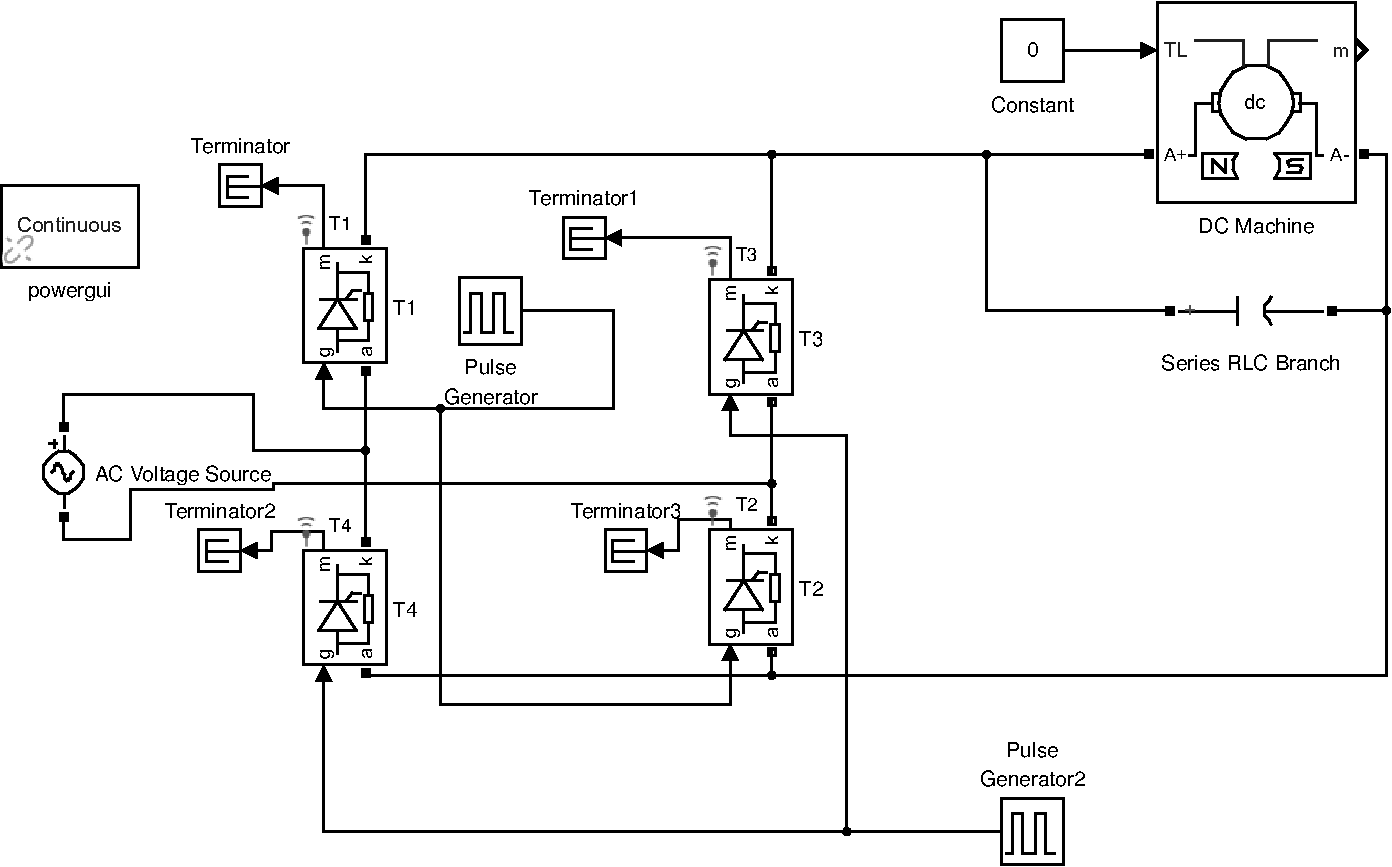
\includegraphics[width=\linewidth]{matlab/sim4}
	\caption{Acionamento de motor DC através de retificador monofásico controlado com filtro capacitivo}
	\label{fig:sim4}
\end{figure}

Rodamos novamente as simulações para ângulos de disparo de $0^\circ$ (figura \ref{fig:res6}) e $90^\circ$ (figura \ref{fig:res7}) (com tensão 24 V rms).

\begin{figure}[H]
	\centering
	\begin{subfigure}[b]{0.49\linewidth}
		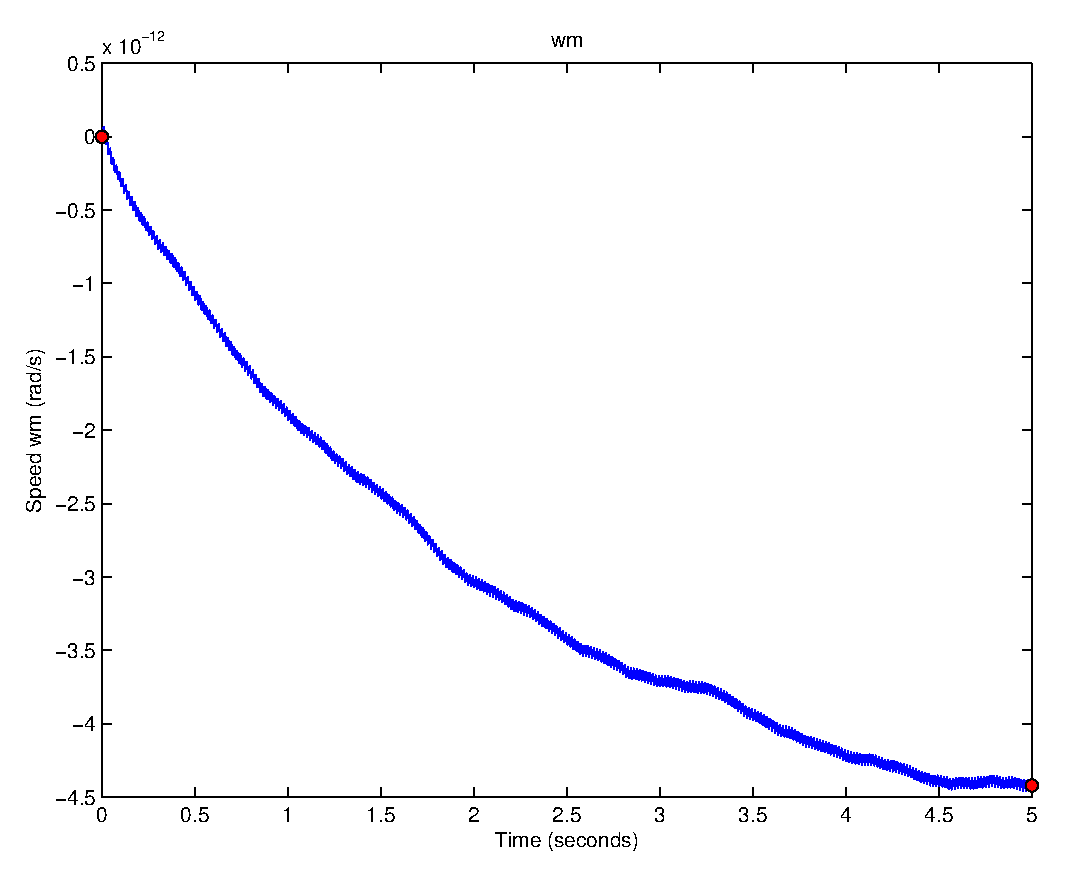
\includegraphics[width=\linewidth]{matlab/wm6}
		\caption{Velocidade Angular}
	\end{subfigure}
	\begin{subfigure}[b]{0.49\linewidth}
		\centering
		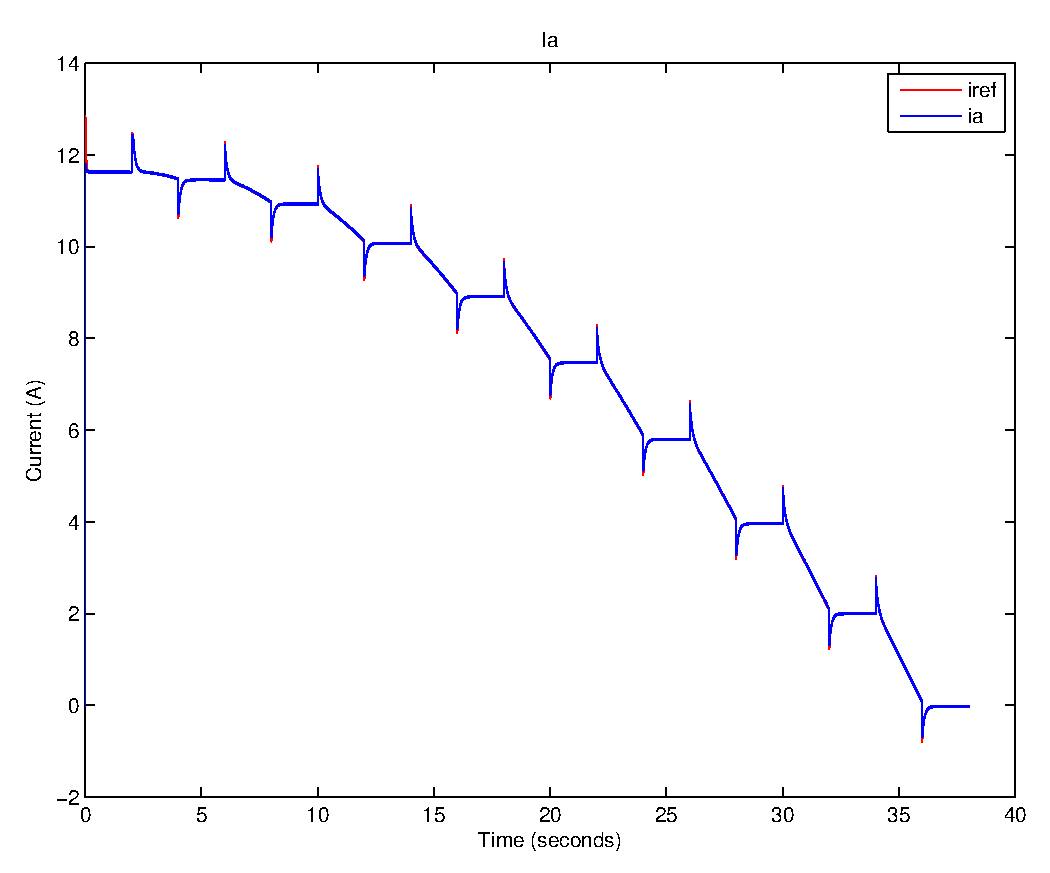
\includegraphics[width=\linewidth]{matlab/ia6}
		\caption{Corrente de armadura}
	\end{subfigure}
	\begin{subfigure}[b]{0.49\linewidth}
		\centering
		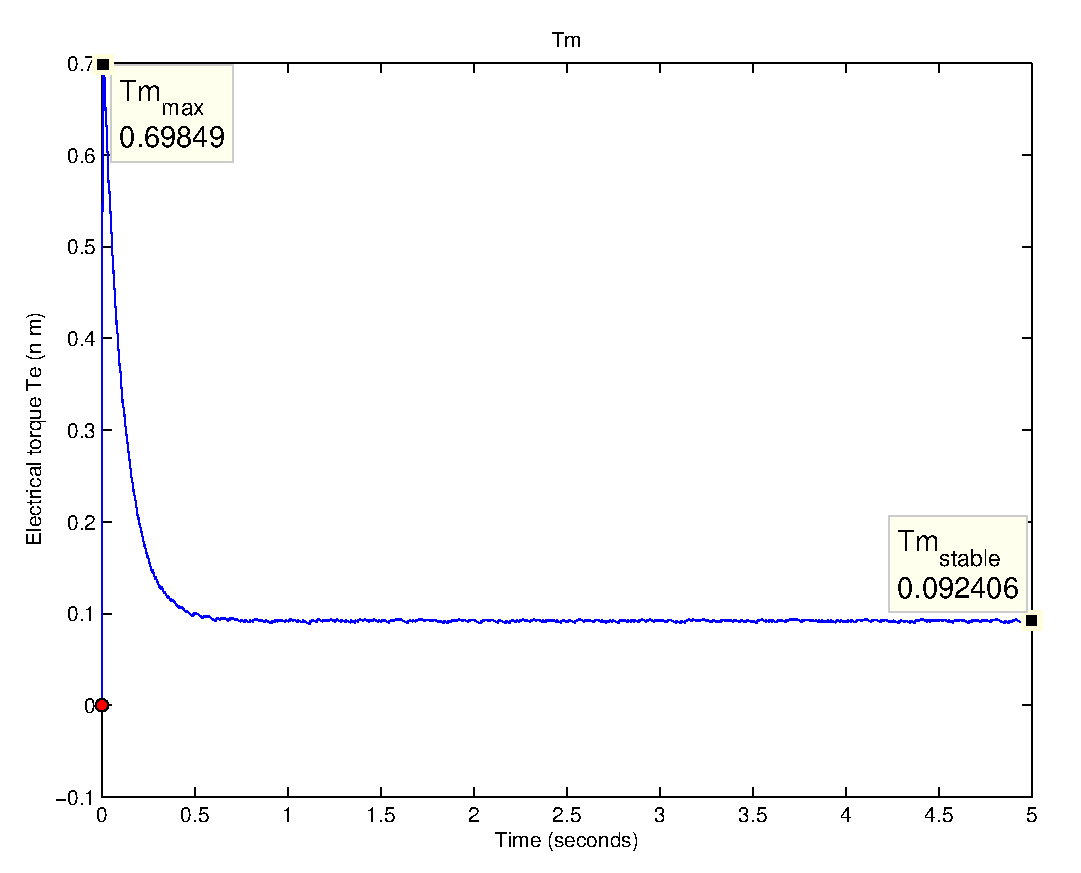
\includegraphics[width=\linewidth]{matlab/tm6}
		\caption{Torque do motor}
	\end{subfigure}
	\caption{Curvas de resposta do motor ângulo de disparo $0^\circ$}
	\label{fig:res6}
\end{figure}

\begin{figure}[H]
	\centering
	\begin{subfigure}[b]{0.49\linewidth}
		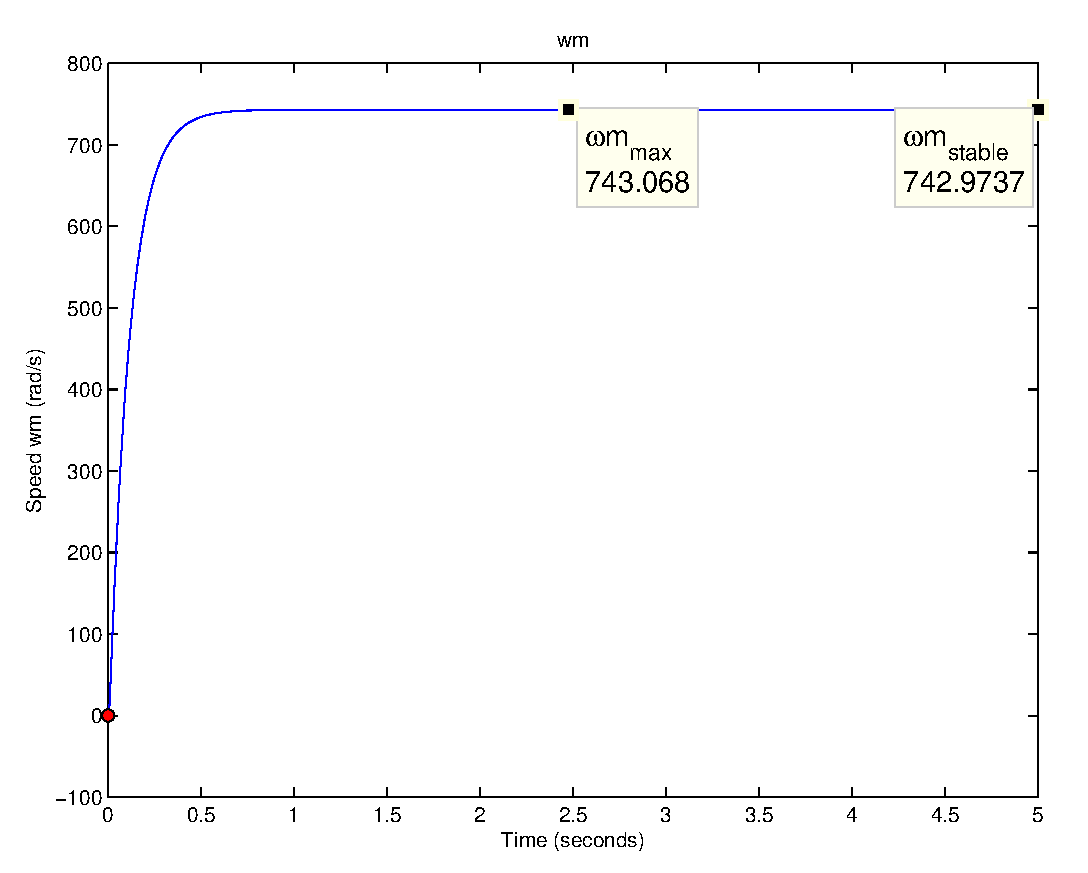
\includegraphics[width=\linewidth]{matlab/wm7}
		\caption{Velocidade Angular}
	\end{subfigure}
	\begin{subfigure}[b]{0.49\linewidth}
		\centering
		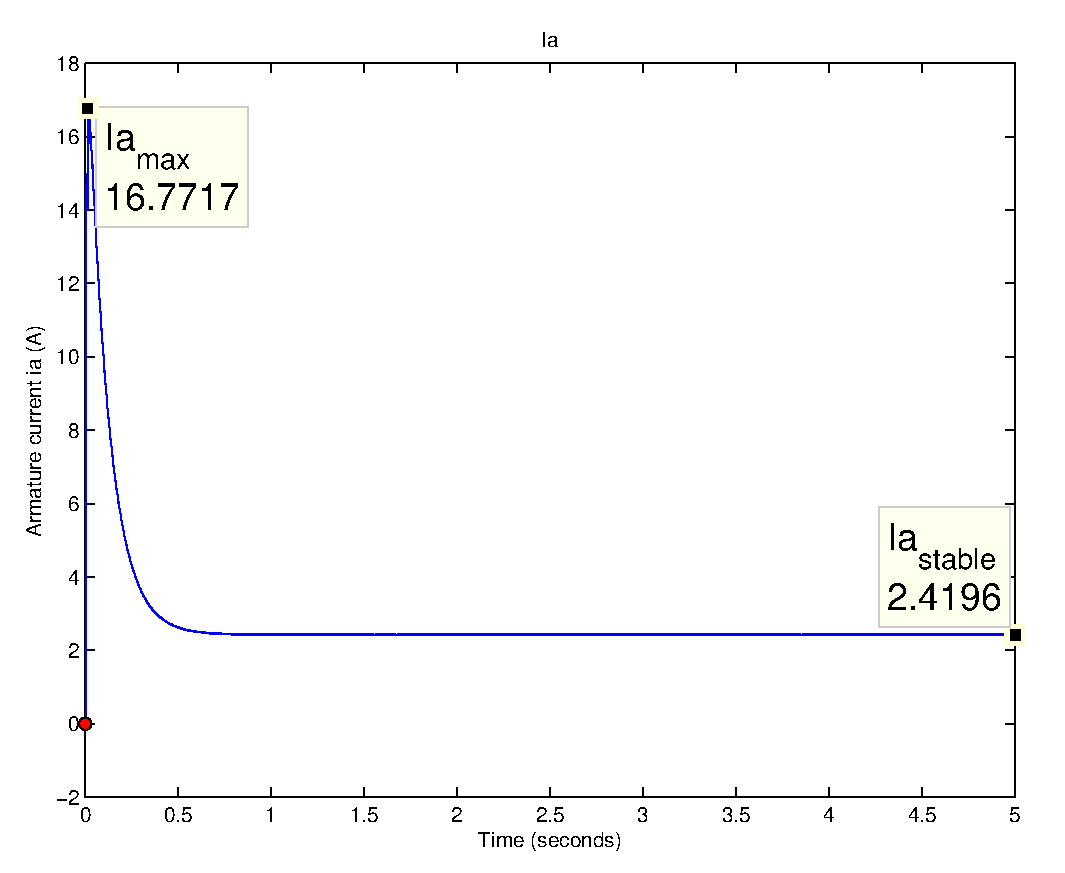
\includegraphics[width=\linewidth]{matlab/ia7}
		\caption{Corrente de armadura}
	\end{subfigure}
	\begin{subfigure}[b]{0.49\linewidth}
		\centering
		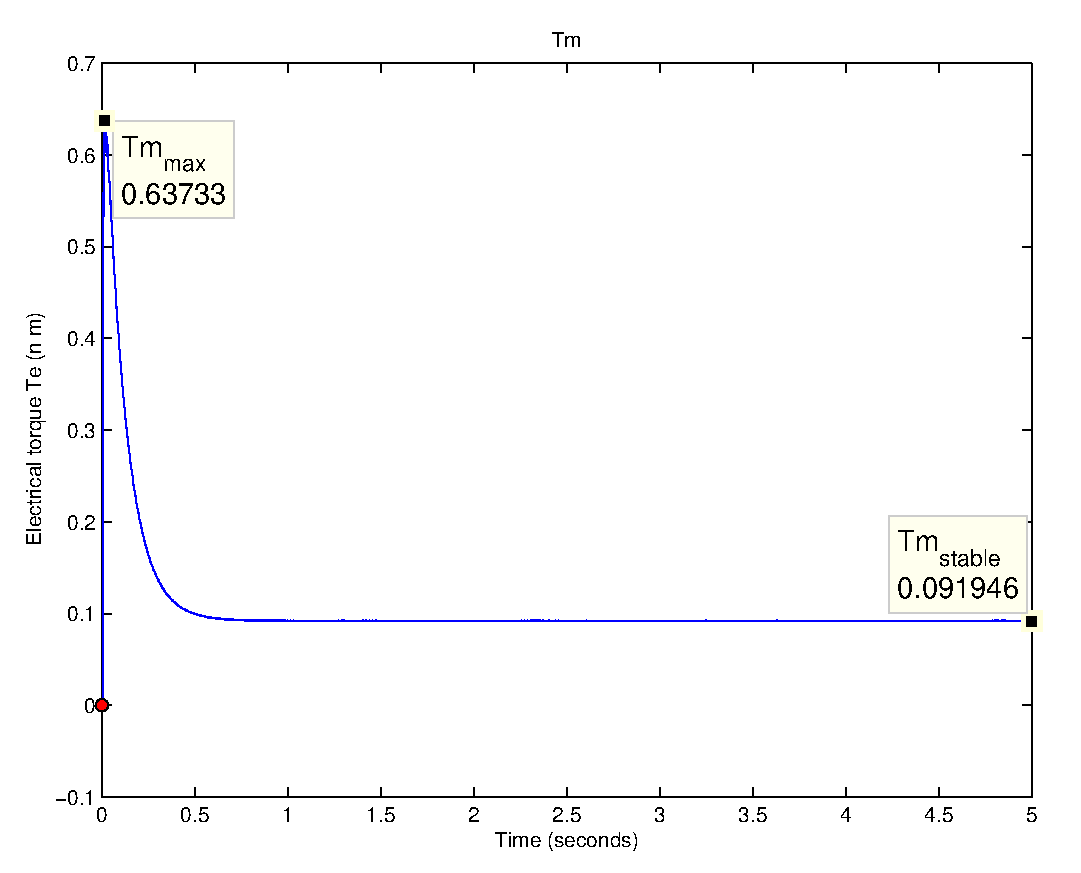
\includegraphics[width=\linewidth]{matlab/tm7}
		\caption{Torque do motor}
	\end{subfigure}
	\caption{Curvas de resposta do motor ângulo de disparo $90^\circ$}
	\label{fig:res7}
\end{figure}
Podemos ver que o filtro conseguiu cortar efetivamente as oscilações na corrente e no torque. Devemos lembrar que o motor é uma carga do tipo RLE, logo a tensão de saída do retificador só assume valores maiores que a tensão gerada pelo motor (E) quando a tensão da fonte é maior que E em valor absoluto. Como essa janela é muito pequena o ângulo de disparo tem pouco efeito no funcionamento do motor uma vez que sua velocidade está alta o suficiente. Uma das dificuldades que encontramos ao rodar essa simulação está relacionada a duração do pulso de disparo do conversor, que dever ser longa o suficiente para que caso a carga E ainda não tenha sido vencida no momento de acionamento, o sinal deve permanecer alto até que essa carga seja superada.

\subsection{Acionamento de motor DC com conversor dual}
Colocamos um circuito de acionamento com conversor dual alimentado por uma fonte alternada (24 V rms@60 Hz) e com um capacitor de 1 F em paralelo com nosso motor, conforme pode ser visto nas figuras \ref{fig:sim5} e \ref{fig:sim6}.
\begin{figure}[H]
	\centering
	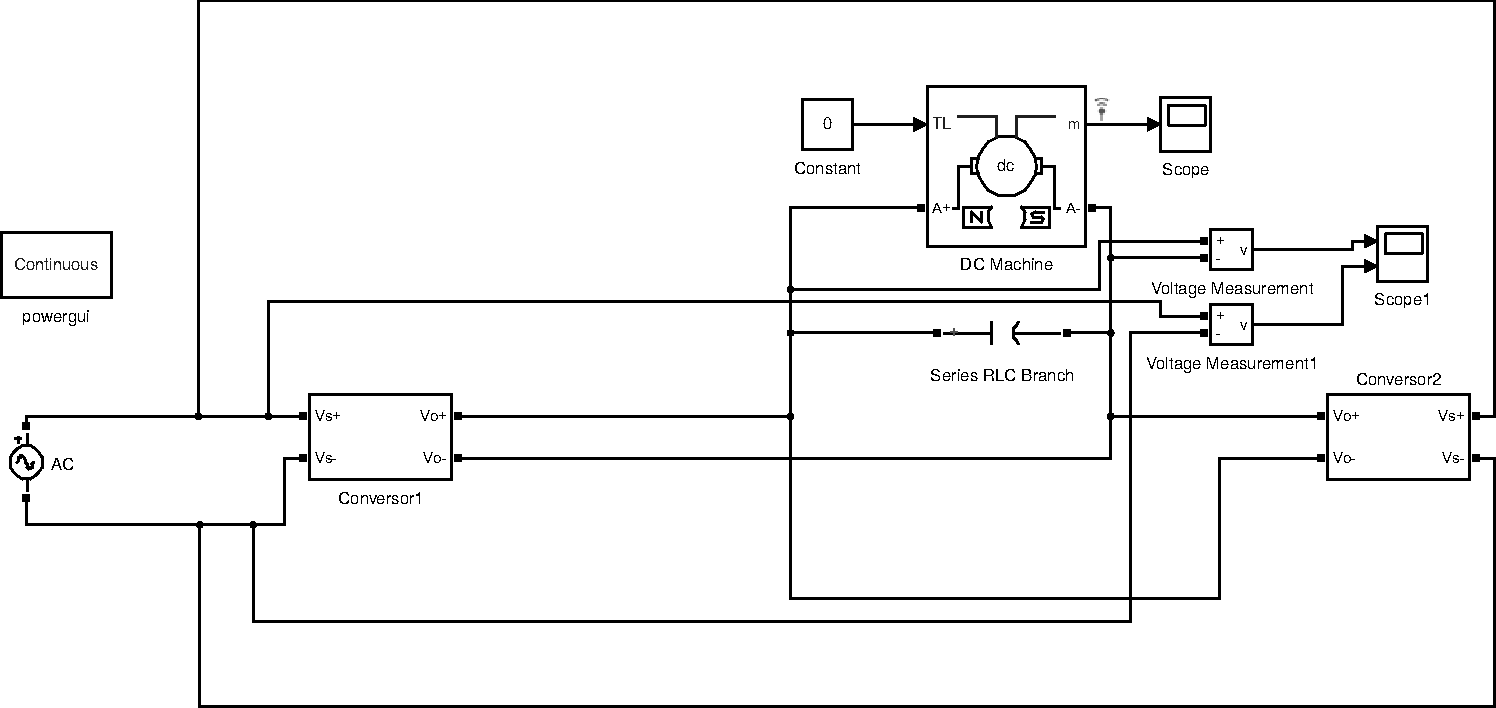
\includegraphics[width=\linewidth]{matlab/sim5}
	\caption{Acionamento de motor DC através de conversor dual}
	\label{fig:sim5}
\end{figure}
\begin{figure}[H]
	\centering
	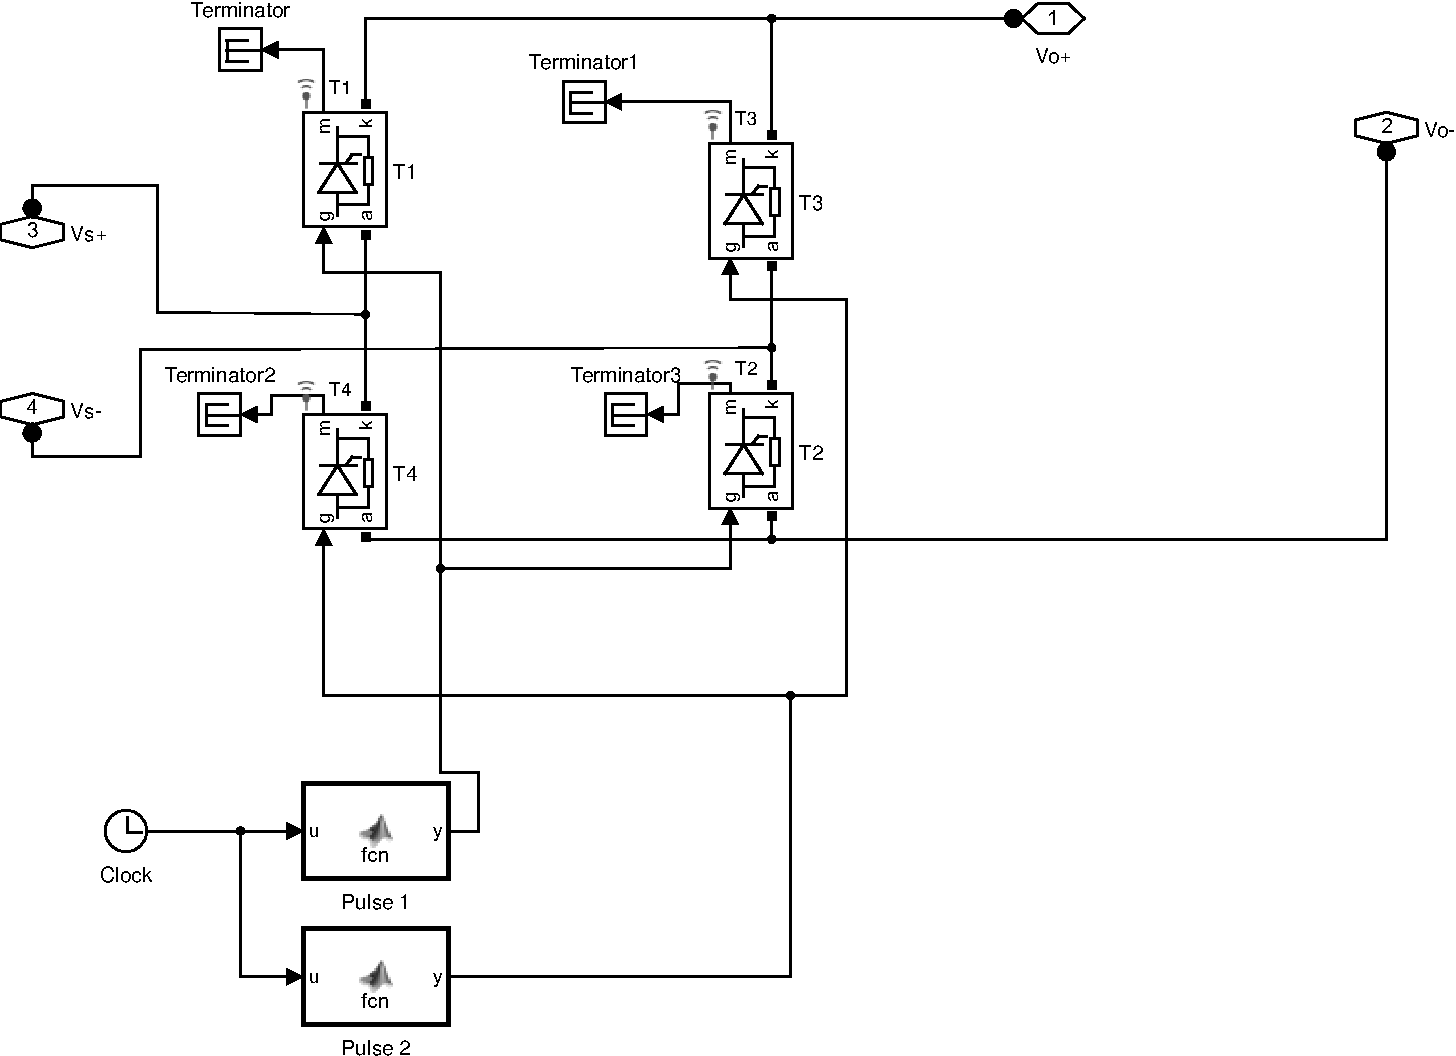
\includegraphics[width=\linewidth]{matlab/sim6}
	\caption{Detalhes do submódulo conversor}
	\label{fig:sim6}
\end{figure}

Simulamos um ciclo completo de operação do motor variando a velocidade de rotação entre os valores máximos direto e reverso segundo o ciclo $\omega = [0,\omega_+,\omega_-, 0]$. Para isso controlamos o ângulo de disparo dos conversores (ativando eles no máximo com o ângulo de disparo $\alpha = 0^\circ$ e desativando com $\alpha = 180^\circ$). Para colocar o motor em rotação máxima positiva ativamos o conversor um com ângulo de disparo $\alpha_1 = 0^\circ$ e o conversor dois com $\alpha_2 = 180^\circ$. Para rotação máxima reversa $\alpha_1 = 180^\circ$ e $\alpha_2 = 0^\circ$ e para freiar basta colocar o mesmo ângulo em ambos conversores, no caso $\alpha_1 = 0^\circ$ e $\alpha_2 = 0^\circ$. Os resultados da simulação estão apresentados na figura \ref{fig:res8}.
\begin{figure}[H]
	\centering
	\begin{subfigure}[b]{0.49\linewidth}
		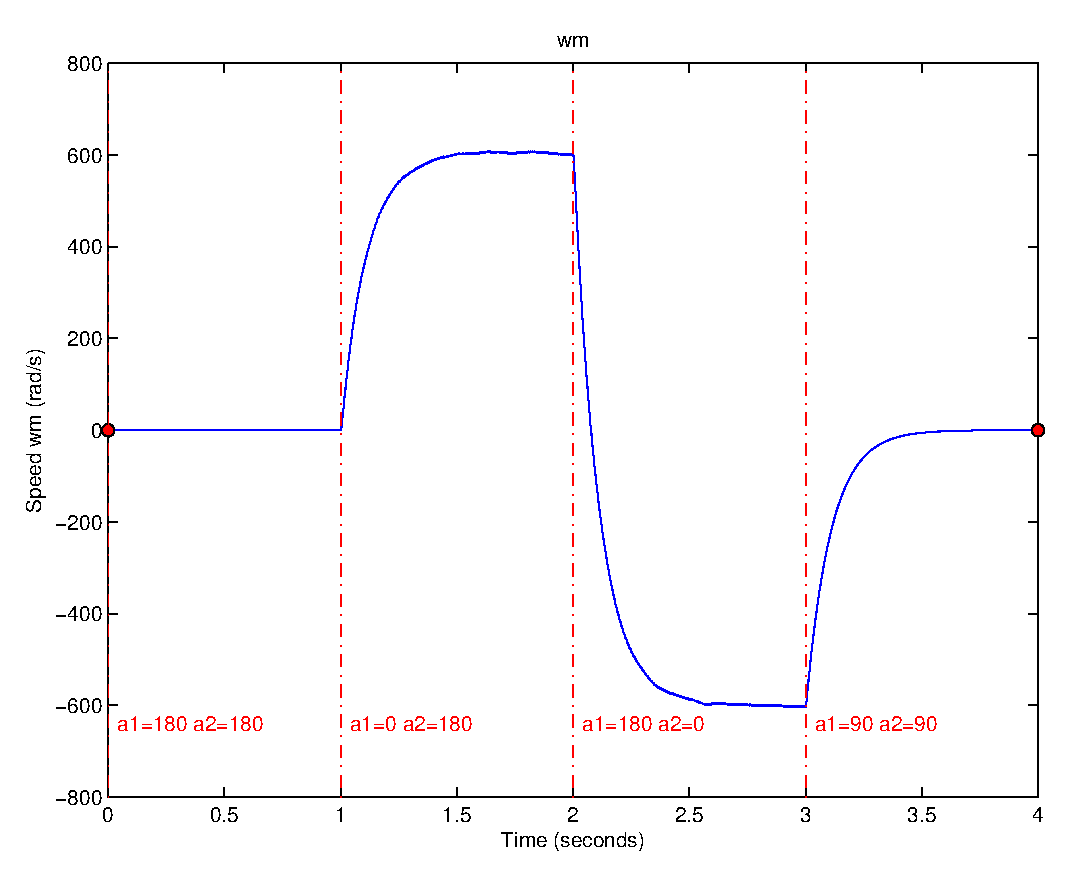
\includegraphics[width=\linewidth]{matlab/wm8}
		\caption{Velocidade Angular}
	\end{subfigure}
	\begin{subfigure}[b]{0.49\linewidth}
		\centering
		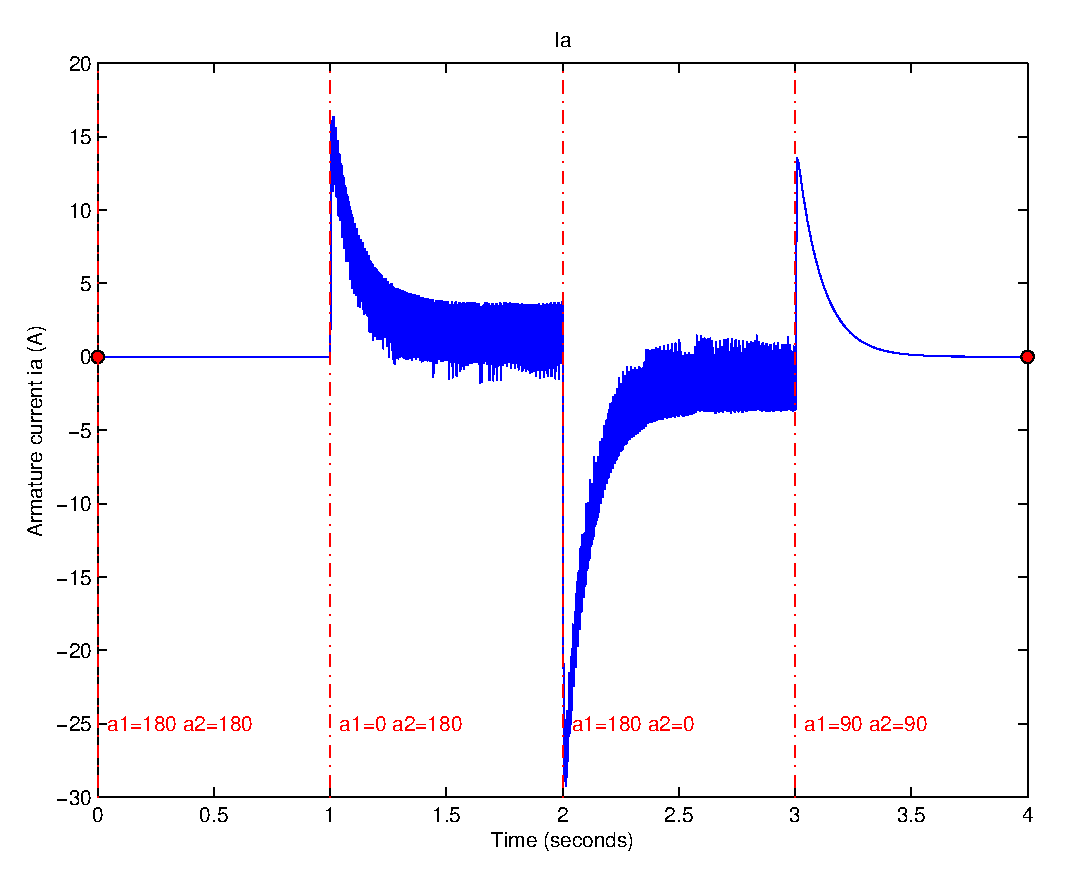
\includegraphics[width=\linewidth]{matlab/ia8}
		\caption{Corrente de armadura}
	\end{subfigure}
	\begin{subfigure}[b]{0.49\linewidth}
		\centering
		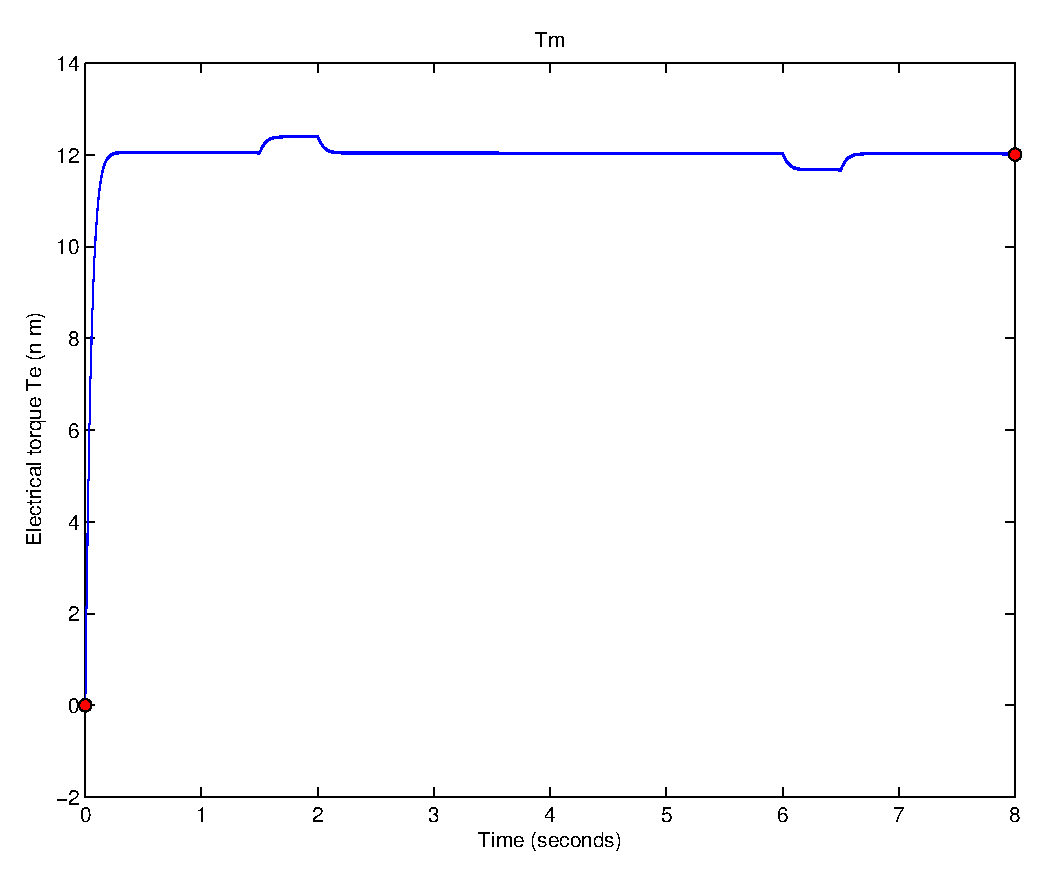
\includegraphics[width=\linewidth]{matlab/tm8}
		\caption{Torque do motor}
	\end{subfigure}
	\caption{Ciclo completo do motor acionado por conversor dual}
	\label{fig:res8}
\end{figure}
Podemos ver o motor operando nos quatro quadrantes nessas figuras.
\section{Questões}
\subsection{Princípio de funcionamento de um motor DC}
Motores DC consistem de dois componentes principais, um rotor e um estator. No rotor existe um enrolamento que conduz a corrente fornecida por uma fonte DC externa, enquanto no estator a excitação de campo é feita por um campo magnético gerado ou através de eletro-ímãs ou através de ímãs permanentes. A corrente de armadura passa através do contato entre as escovas fixas e os anéis coletores e sua interação com o campo magnético gerado pelo estator cria uma força que faz o rotor girar até que as forças em cada lado do rotor se alinhem. Quando essa condição está para ser atingida o sentido da corrente nos enrolamentos é invertida através dos comutadores, que nada mais são do que uma segmentação nos anéis coletores. Ao se utilizar vários pólos conseguímos transformar nosso torque de rotação em algo aproximadamente constante.
As equações que regem o funcionamento de um motor DC (conforme apresentadas em \cite{bb:mohan}) são as seguintes:
\begin{equation}
	v_a(t) = R_ai_a(t) + L_a\frac{d i_a(t)}{dt} + e_a(t)
\end{equation}
\begin{equation}
	T_{em}(t) = J \frac{d\omega_m(t)}{dt} + B\omega_m(t) - T_{WL}(t)
\end{equation}
\begin{equation}
	e_a(t) = K_E\phi_f\omega_m(t)
\end{equation}
\begin{equation}
	T_{em}(t) = K_t\phi_fi_a(t)
\end{equation}
Para motores por eletroímã:
\begin{equation}
	\phi_f = k_fi_f
\end{equation}
Para motores de ímã permanente:
\begin{equation}
	\phi_f = cte
\end{equation}
Onde
\begin{itemize}
	\item $i_a$ é a corrente de armadura;
	\item $e_a$ é força contraeletromotriz;
	\item $T_{em}$ é o torque do motor;
	\item $T_{WL}$ é o torque da carga;
	\item $R_a$ é a resistência da armadura;
	\item $L_a$ é a indutância da armadura;
	\item $J$ é a inércia do motor;
	\item $B$ é o atrito do motor;
	\item $K_E$ é a constante elétrica do motor;
	\item $K_T$ é a constante de torque do motor;
	\item $i_f$ é a corrente de campo;
	\item $\phi_f$ é o fluxo de campo;
	\item $k_f$ é a constante de campo do motor;
\end{itemize}

Em um motor DC é possível maximizar o torque ajustando o fluxo eletromagnético nos enrolamentos de campo $\phi_f$ para que o motor opere abaixo da velocidade nominal. Nessas condições conseguimos travar o torque no seu valor nominal ajustando a tensão aplicada nos terminais da armadura $V_a$.

Para trabalhar com velocidade maior do que a velocidade nominal, travamos $V_a$ em seu valor nominal, abaixando o fluxo de campo $\phi_f$. Nesse modo o torque vai cair com a queda de $\phi_f$. Ao travar a corrente de armadura $I_a$ e a tensão $V_a$ em seus valor nominais podemos então trabalhar na região de potência constante e conseguimos atingir velocidades maiores do que a nominal, ao custo de quedas no torque obtido.

Notamos então que no modo de torque constante, conseguimos controlar a velocidade do motor variando a tensão aplicada nos terminais de armadura e para o modo de potência constante conseguimos ajustar o valor do torque e da velocidade ao variar o fluxo de campo, que é uma função da tensão e da corrente nos terminais do circuito de campo $V_f$ e $I_f$.

\subsection{Quadrantes dos conversores}
O conversor monofásico controlado de onda completa opera somente em dois quadrantes uma vez que ele não permite a inversão da corrente aplicada no motor. Já o conversor dual opera nos quatro quadrantes, conforme podemos ver no ciclo completo de operação mostrado na figura \ref{fig:res8} em que vemos aceleração direta, reversa e frenagem.

\subsection{Controle em malha aberta}
Uma estratégia para controle em malha aberta do motor utilizando o conversor dual seria dado o valor absoluto da velocidade de referência $\omega*$, ajustar o ângulo $\alpha$ de disparo entre $0^\circ$ e $180^\circ$ (sendo que quanto maior é $\omega*$ menor deve ser $\alpha$). Utilizaríamos esse ângulo para disparar um dos conversores enquanto desativamos o outro (desativar um conversor é equivalente a dispará-lo com um ângulo de $180^\circ$), a escolha de qual conversor seria feita através do sinal de $\omega*$.
\bibliography{mybib}
\end{document}

